%%%%%%%%%%%%%%%%%%%%%%%%%%%%%%%%%%%%%%%%%%%%%%%%%%%%%%%%%%%%%%%%%%%%%%%%%%%%%%%%
%2345678901234567890123456789012345678901234567890123456789012345678901234567890
%        1         2         3         4         5         6         7         8

\documentclass[letterpaper, 10 pt, conference]{ieeeconf}  % Comment this line out if you need a4paper

%\documentclass[a4paper, 10pt, conference]{ieeeconf}      % Use this line for a4 paper

\IEEEoverridecommandlockouts                              % This command is only needed if 
                                                          % you want to use the \thanks command

\overrideIEEEmargins                                      % Needed to meet printer requirements.

% See the \addtolength command later in the file to balance the column lengths
% on the last page of the document

% The following packages can be found on http:\\www.ctan.org
\usepackage{subfig}
\usepackage{graphicx} % for pdf, bitmapped graphics files
%\usepackage{epsfig} % for postscript graphics files
%\usepackage{mathptmx} % assumes new font selection scheme installed
%\usepackage{times} % assumes new font selection scheme installed
%\usepackage{amsmath} % assumes amsmath package installed
%\usepackage{amssymb}  % assumes amsmath package installed
\usepackage{url}
\usepackage{array}
\usepackage{tabularx}
\usepackage{tabulary}
\usepackage{booktabs}


\title{\LARGE \bf
Bringing robotics in formal education \\
using the Thymio open source hardware robot
}


\author{Francesco Mondada$^{1}$, Michael Bonani$^{2}$, Fanny Riedo$^{2}$, Manon Briod$^{1}$, \\
L\'ea Pereyre$^{1}$, Philippe R\'etornaz$^{1}$ and St\'ephane Magnenat$^{1}$% <-this % stops a space
\thanks{*This research was partially supported by the Swiss National Center of Competence in Research ``Robotics'' (Thymio robot development and deployment), partially by GebertRuf Stiftung (design of accessories), partially by the Swiss NSF project CRAGP2 151543 ``Robotics in schools'', and partially by the EU-FP7 project ASSISIbf, no. 601074 (survey on open hardware). Many thank to Luc Bergeron and his team at écal.ch for the industrial design of Thymio; Didier Roy, David Sherman and all the INRIA team for their contributions and diffusion in France; Gordana Gerber for the educational material; all the Mobsya team for the effort in production and sale.}% <-this % stops a space``anyone''
\thanks{$^{1}$Francesco Mondada, Manon Briod, L\'ea Pereyre, Philippe R\'etornaz and St\'ephane Magnenat are with the Laboratoire de Syst\`emes Robotiques,
        Ecole Polytechnique F\'ed\'erale de Lausanne (EPFL), Switzerland
        {\tt\small firstname.lastname@epfl.ch}}%
\thanks{$^{2}$Michael Bonani and Fanny Riedo are with Mobsya Association, Ecublens, Switzerland
        {\tt\small michael.bonani@mobsya.org} and {\tt\small fanny.riedo@mobsya.org}}%
}


\begin{document}



\maketitle
\thispagestyle{empty}
\pagestyle{empty}


%%%%%%%%%%%%%%%%%%%%%%%%%%%%%%%%%%%%%%%%%%%%%%%%%%%%%%%%%%%%%%%%%%%%%%%%%%%%%%%%
%%%%%%%%%%%%%%%%%%%%%%%%%%%%%%%%%%%%%%%%%%%%%%%%%%%%%%%%%%%%%%%%%%%%%%%%%%%%%%%%

%\begin{abstract}
%Mobile robots are interesting tools for education because of both the enthusiasm they raise and the multidisciplinary nature of their technology.
%However, because of their price, complexity, bias towards specific groups (boys), and unproved educational value, they are still seldom used in schools and edutainment.
%This paper presents a system-design approach and the resulting Thymio robot that tackle these problems in a holistic way.
%We show how this strategy achieved a low price leading to a high demand and raising the interest of teachers.
%The robot and its development environment are open source and the whole project follows an open distribution and participative model.
%Finally, we show deployment statistics proving that the robot is gender- and age-neutral and preliminary results towards assessing the educational value of robots.
%\end{abstract}


\section{Introduction}

Mobile robots are interesting tools for education because of both the enthusiasm they raise and the multidisciplinary nature of their technology.
Because autonomous mobile robots sense the environment and take actions based on their perception, they seem to display \emph{intentions of their own}.
This fascinates the users of the robot and creates feelings of accomplishment and power in the creators.
The permeating presence of robots in science fiction and their projected use in our society increases these emotions by giving a sense of touching the future. % SM: not so happy with my sentence here
Children can spend hours looking at a robot interacting with its environment and adults can approach robots as a new hobby that replaces radio and electronics kits.
Robots embed various technologies and therefore give access to a wide range of fields, such as complex mechanics, sensors, wireless transmission, mathematics, computer science, etc.
The emotional potential of mobile robots and their varied technology makes them the ideal tool for education at large.

Despite this potential, robots are still not widespread in schools as they could be and this for several reasons. Among them we can mention:
\begin{enumerate}
\item Although there are many robotic projects developing innovative and interesting educational robots, few reach a sufficient maturity to become distributed and accessible to schools. 
\item A robot performing interesting behaviors is a complex piece of technology and therefore expensive. 
Indeed, for having an educational value and providing an interesting level of interaction, a robot must embed a wide set of sensors and actuators.
Existing platforms with these features cost several hundred Euros.
This prevents most schools, which have a limited budget for equipment, to acquire interesting robots.
\item Introducing robotic tools into teaching activities requires investment in time and training for the teachers.
In Europe, despite a trend in including more and more technological tools into the learning process, teachers are still insufficiently trained and are reluctant to introduce these tools in their teaching activity~\cite{CERI2008}.
To be accepted by teachers, robots must be therefore both accessible with minimal effort and be associated with-well prepared educational material. 
Moreover an infrastructure should allow the exchange of educational material among the teachers.
\item Robot construction, use, and programming is often perceived as a boyish activity in our society~\cite{leonard2009lego,nourbakhsh2009robot}.
% For instance, several authors report that girls have such a perception of the LEGO Minstorms~\cite{leonard2009lego,nourbakhsh2009robot}.
This strongly limits the potential of robots as general-purpose educational tools, especially in schools.
\item Finally, many teachers are reluctant to follow volatile trends, especially if based on purely commercial arguments. Teachers prefer to invest in stable tools, and this is the opposite of todays consumer technology, often very volatile and based on continuos renewal rather than on durability.
\end{enumerate}

Open source hardware projects can address several of these issues in a different way than pure commercial products. 
By open source hardware we understand, following the definition of the Open Source Hardware Association\footnote{\url{http://www.oshwa.org/definition/}}, ``hardware whose design is made publicly available so that anyone can study, modify, distribute, make, and sell the design or hardware based on that design''.
In this paper, we show that this concept, implemented as a project in a community of users, developers and producers, brings a very interesting added value to the robot and to the educational methods. 
This is illustrated by the results achieved with Thymio and is compared with the feedback of a group of robotics engineers active in open source hardware design.
We can well observe both similarities and differences between our education-centered project and other open source robotic hardware projects, pointing to challenges and opportunities.
More details on the robot and the related results can be found in~\cite{RiedoPhD, magnenat2014}.  

\section{Related Work}

There is a very large number of publications presenting educational robots with different prices and features, from very low-cost systems targeting, for instance, education in Africa~\cite{Rubenstein2015,Gyebi2015} to extremely sophisticated humanoids~\cite{Hood2015,Mazzoni2016}.
Among those, only very few are commercially available, limiting their validation by education scientists.
This results in 90\% of publications about validation of educational results made on LEGO\textsuperscript{\textregistered} Mindstorms\textsuperscript{\textregistered}~\cite{benitti2012exploring}.
The LEGO\textsuperscript{\textregistered} Mindstorms\textsuperscript{\textregistered} EV3\footnote{\url{http://mindstorms.lego.com}} is expensive ($\approx$ 400\,\$) but offers a wide range of possibilities, especially at the mechanical level using LEGO\textsuperscript{\textregistered} bricks and at the software level with its graphical programming environment. 
At a lower price, LEGO\textsuperscript{\textregistered} proposes the WeDo\textsuperscript{\textregistered} system ($\approx$ 80\,\$).
The WeDo\textsuperscript{\textregistered} is similar to EV3 but only reads one sensor and controls one actuator and must always be connected to a desktop computer.
The BeeBot robot\footnote{\url{http://www.beebot.org.uk}} is a cheap ($\approx$ 90\,\$) autonomous system.
However, it is not a real robot but rather an automaton: There is no perception of the environment, just a good encoder for precise movements and a simple programming interface based on buttons giving directions for the movements.

Among these widely used robots, none is part of an open source hardware project.
The only effort in this direction comes from LEGO\textsuperscript{\textregistered}, that made public all the schematics of the EV3 in an hardware developer kit, to allow the design of extensions. 
Otherwise, only few educational robots are both used in schools and are issued from an open hardware project:
Scribbler2, produced and sold by Parallax\footnote{\url{http://www.parallax.com}} ($\approx$ 180\,\$), is a 188~mm large robot, designed to run on the ground and equipped with few light sensors, one distance sensor, two ground sensors and few LEDs display.
It runs on standard AA batteries and has a hacker port for interfacing electronic extensions.
It is programmable with a graphic or text code interface.  
The main weakness of Scribbler2 is its performance per price ratio and the limited compatibility with other systems. 
Moreover there seems to be no real community around its development.
The e-puck~\cite{mondada2009puck} robot is a robot targeting university-level education.
Well equipped with sensors and actuators, modular and compact, it can be programmed with professional environments.
Several simulators allow to run experiments of high complexity. 
There is an active community of users and developers around it.
It's main weakness is its high price ($\approx$ 870\,\$).
Finch\footnote{\url{http://www.finchrobot.com/}} ($\approx$ 99\,\$) is a very simple robot that has been designed around a wired connection to the computer. 
This connection reduces electronics requirements, such as batteries or wireless communication, and allows to implement the control entirely on the computer.
This results in a very broad set of possible programming languages available, the real force of this robot. 
On the other hand the cable does not allow real autonomy and mobility of the robot.
Finally the mBot\footnote{\url{http://www.makeblock.cc/mbot/}} is a mobile platform based on the Arduino board. 
The very cheap and simple electronics allow to drastically reduce the price of the system ($\approx$ 75\,\$) but also reduces the perception possibilities to a couple of sensors. 

In respect to these robots, Thymio has a compact size (120~mm), many interaction possibilities, an affordable price and a large set of sensors.
It's design makes the best use of the recent cheap components coming from the explosive growth of the mobile devices market. 
To the best of our knowledge, beside Thymio there are no educational products exploiting this and providing many sensors and actuators at a price below 130\,\$.

Among the main target users there are teachers.
For teachers, the motivation to use robotic tools in their classes depends on many factors \cite{chevalier2016}.
Among them, the availability of material and training plays a key role.
The BeeBot mentioned previously, because of its radical simplicity, is one of the tools that needs the least training. 
Moreover its use in learning activities is based on a simple grid on a printed mat on the ground, allowing fast and easy integration in existing lessons.
These are probably two important factors for its success in schools~\cite{2008highfield,2008demichele} and the availability of a rich set of educational material\footnote{\url{https://www.learningplace.com.au/deliver/content.asp?pid=38840} and \\ \url{http://beebots.skola.edu.mt/}}.
However, the total lack of sensors reduces the BeeBot to an automaton, easy to use but limited to very simple activities for young kids, without much potential in teaching computational thinking or robotics concepts.

For more complex robots, both the development of educational material and the training of teachers require a very important effort, needing a good mix between robotics and educational skills. 
Moreover, educational material changes very much from school to school, as education is very dependent from local educational programs and languages, for instance. 
In the particular case of Switzerland, for instance, every of the 26 states composing the confederation has its own school program and its own language among the four national ones. 
Educational material and the related training have therefore to be adapted to each situation, which requires a huge effort.
Even for large companies like LEGO\textsuperscript{\textregistered} this development is not affordable. 
A solution is to have an active community of users contributing to the development of the material in a distributed manner, adapting the material to the local situation.
LEGO\textsuperscript{\textregistered} itself is moving in the direction of promoting communities of users \cite{Hienerth2014} with a user-producer interaction close to those of open hardware projects.
The open source community regrouping developers, producers and final users is therefore a very interesting model to address the distributed development and sharing of educational material, and the diffusion of training sessions.
This model is an extension to education of what already practiced in projects like Arduino~\cite{Jamieson2010}.

%Several initiatives have focused on increasing the rate of females in engineering in general and in robotics in particular~\cite{weinberg2007impact}.
%Roberta~\cite{2010bredenfeld} is one of the largest and uses the LEGO Minstorms.
%Recent work has shown that a different approach to robotics, for instance linking with arts and proposing creative workshops~\cite{nourbakhsh2009robot}, can improve the attractiveness for girls. 
%Some researchers have created hardware tailored to crafting activities, such as the PicoCricket~\cite{2008rusk} which is close to the NXT but does not require LEGO construction.
%Compared to these works, Thymio aims at being attractive for both genders.

%Several studies have measured the impact of the use of robots on children~\cite{weinberg2007impact,nourbakhsh2009robot,sinkele2010effectiveness}, but none of these provide quantitative data on the usage of the different features of the robot.
%On the contrary, Thymio can log the usage of its features, providing a tool to monitor the progress of children and to investigate the value of different curricula.


\section{Design choices}

\begin{figure}
   \centering
	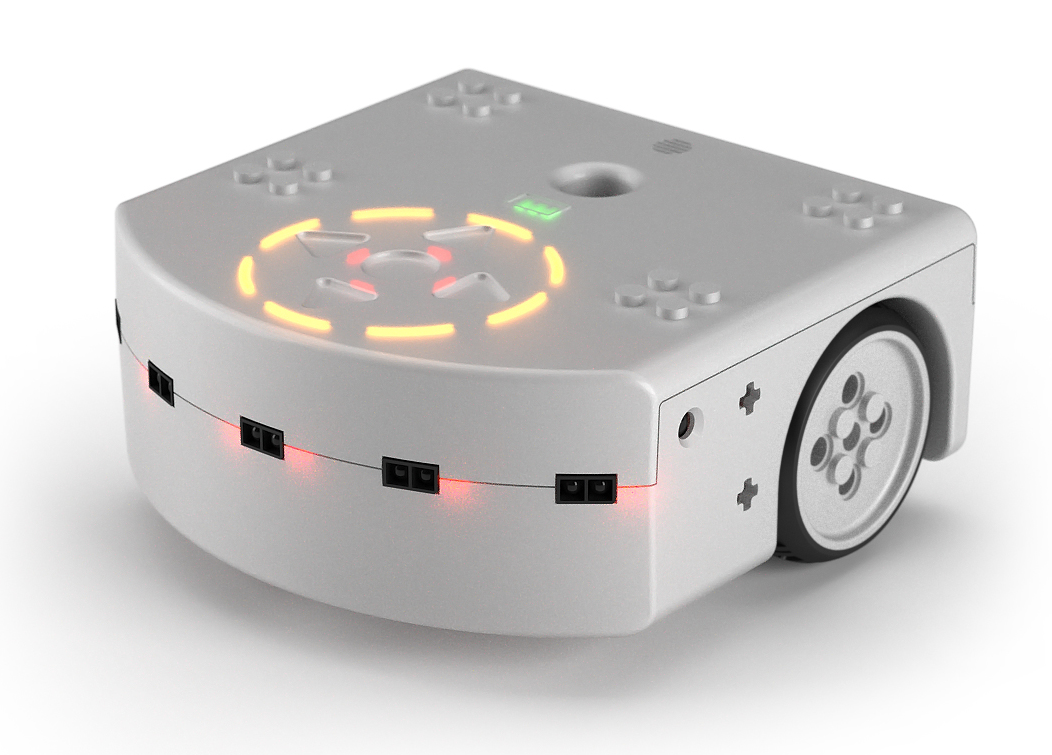
\includegraphics[width=.8\columnwidth]{figures/front_2016}
	\vskip 1.5em
	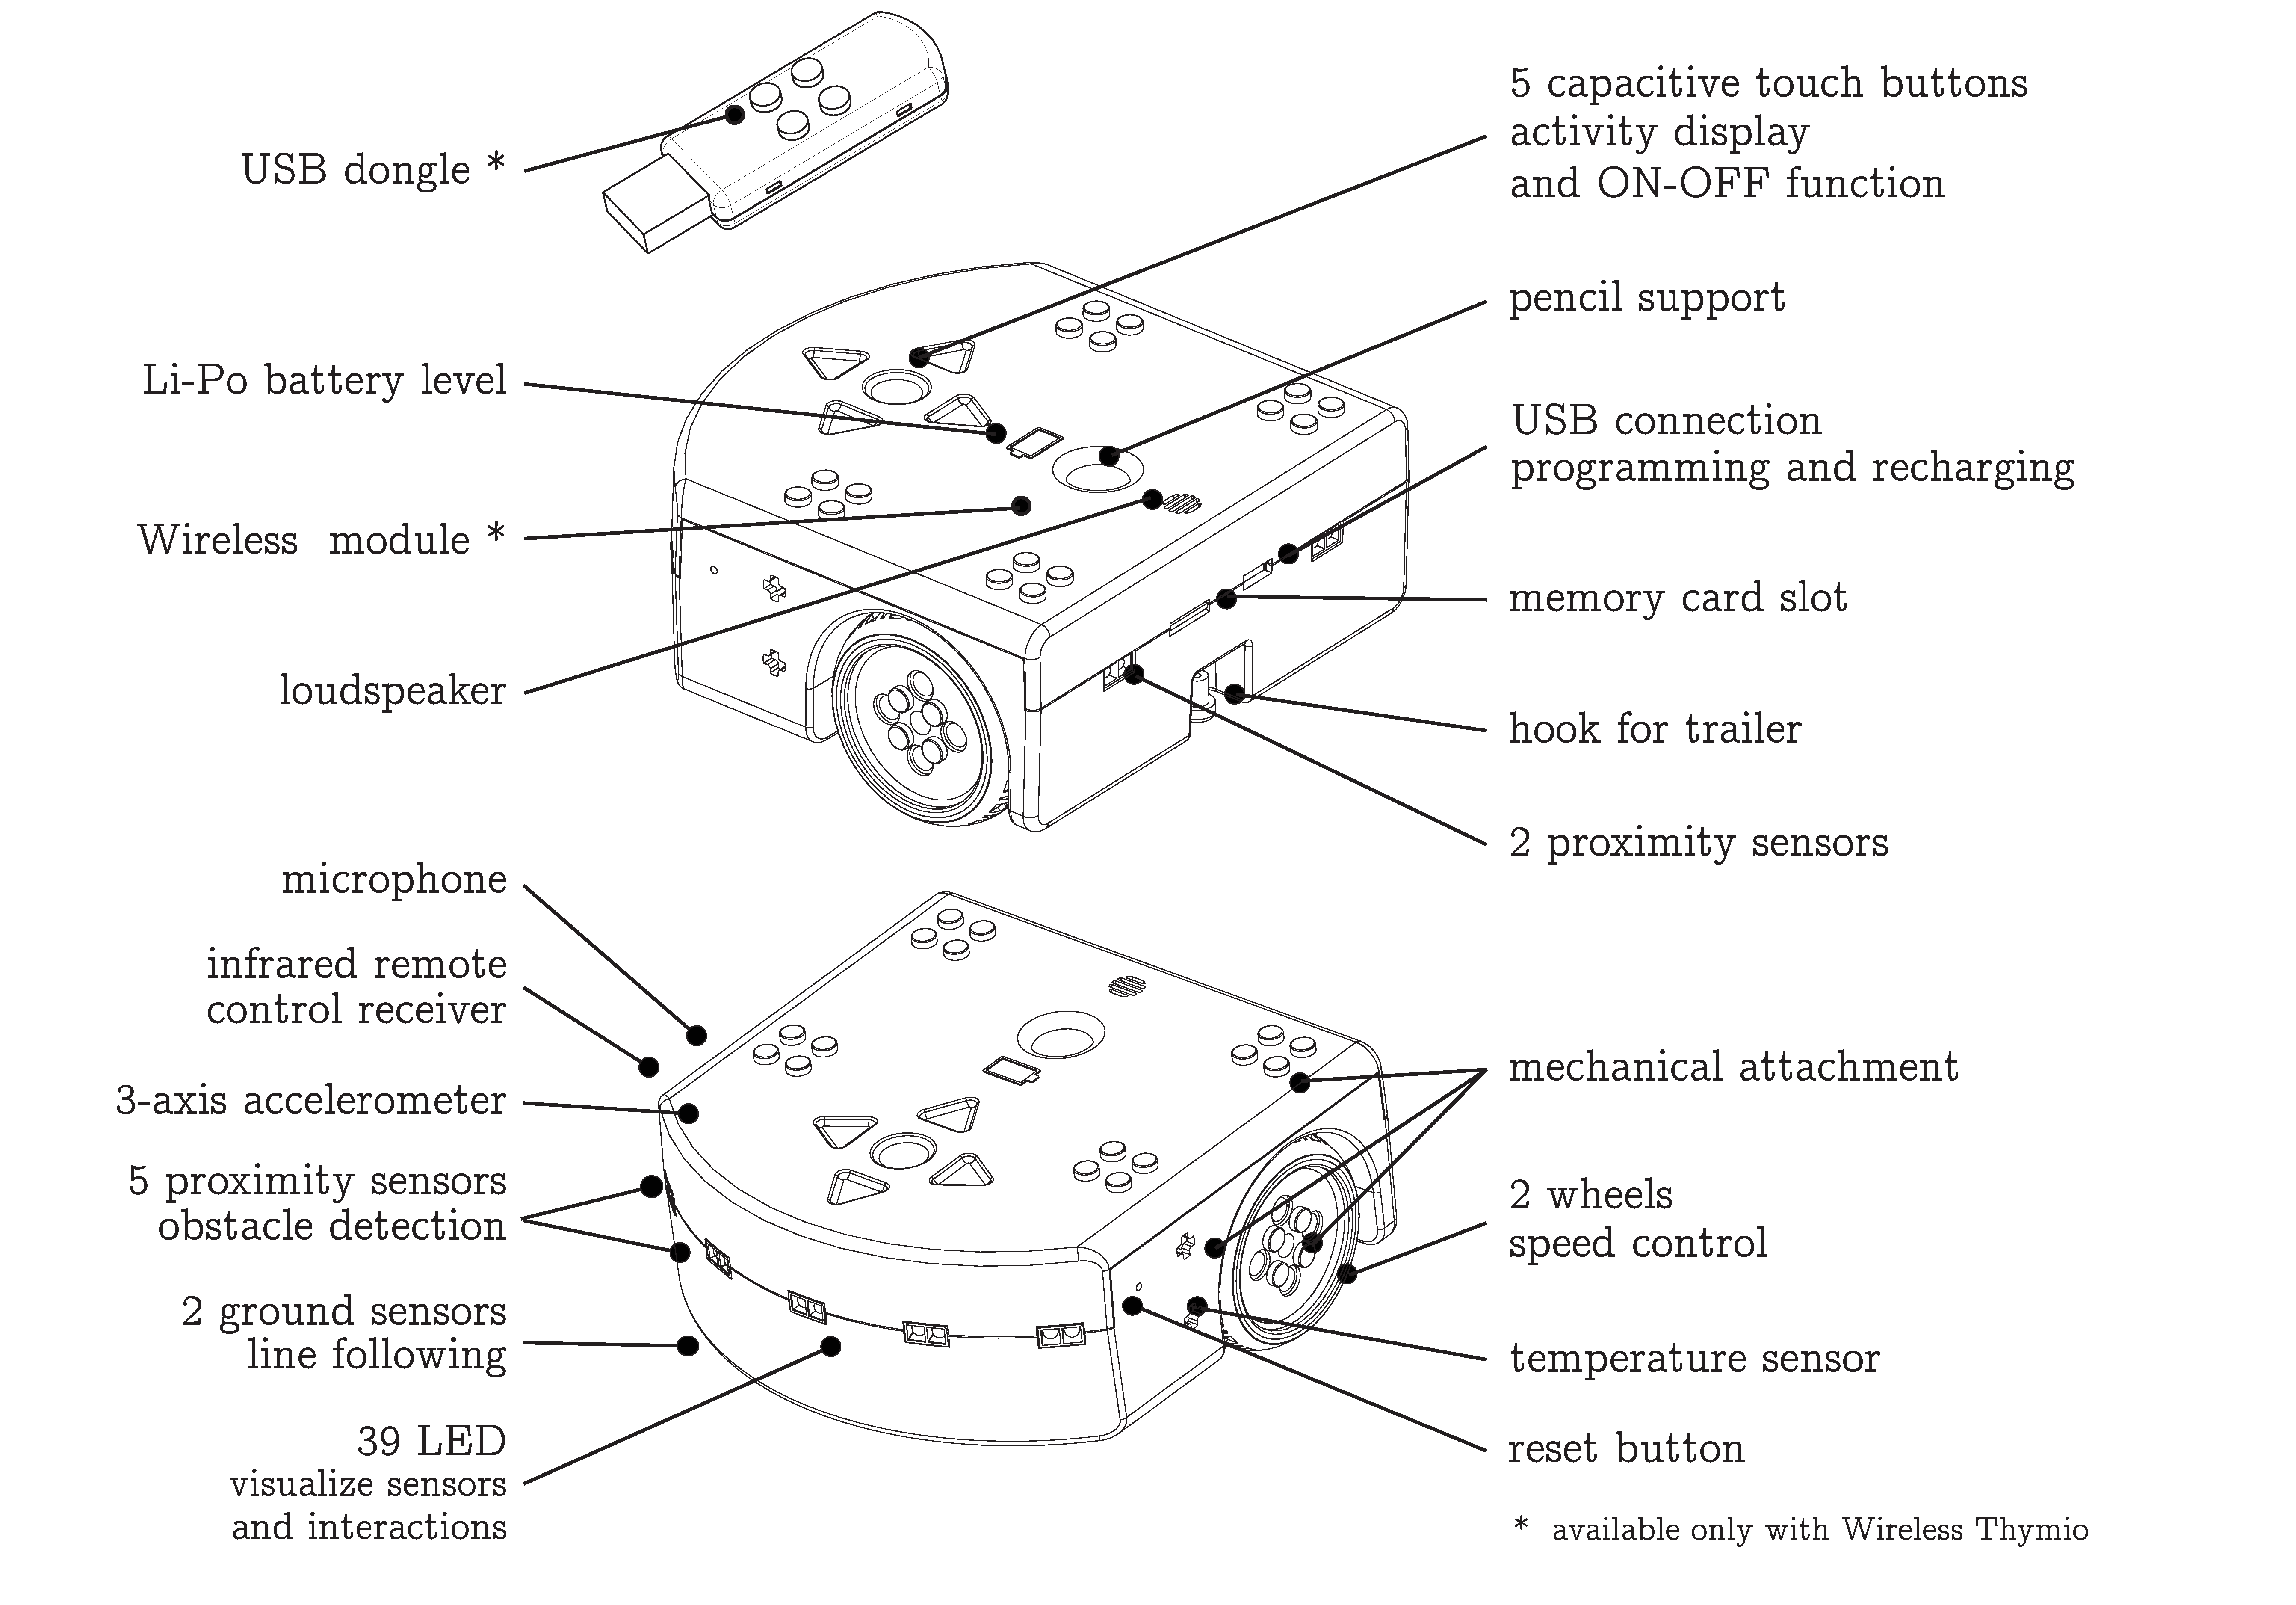
\includegraphics[width=\columnwidth]{figures/wirelessThymioVecto}
	\caption{The Thymio robot and its main components for the Wireless and the plain version.}
	\label{fig:schematique}
\end{figure}


We designed the Thymio robot along seven main axes: a low price to address a larger number of users, a feature set that suits both genders and multiple ages from young children to adults, a combination of sensors, actuators, and programming features that facilitates learning, a mechanical design that allows creative extensions by the users themselves, a set of ready-to-use behaviors to get a demonstration right out of the box, an accessible programming environment, and an open source  community contributing to the design and disseminating the results.
The result is a miniature (10\,cm in diameter, see Figure~\ref{fig:schematique}) differential-wheeled robot suited for use on a desktop.
The robot is robust enough to be mishandled by children, as it can fall from a table without breaking itself.
It features a translucent white hull and a wide range of sensors and actuators (see Figure~\ref{fig:schematique} bottom).
The robot embeds a battery, rechargable by \textsc{usb}, that provides an autonomy of about 2 hours.

We start by presenting here the first six main axes, before moving to the next section devoted the open hardware specificities.

\subsection{Low Price}

Our main concern during the mechatronic design of Thymio was to keep a low production cost. 
Price is a key factor for the adoption of the robot by schools~\cite{kradolfer2014sociological}.
In our previous experience with designing robots, most of the costs was due to the electronics and the sensors~\cite{thesis_michael}, not to the mechanical parts.
As we wanted Thymio to be an affordable robot, we selected electronic components with great care and explored different design solutions in order to limit the number of expensive components.
In particular, we focused on low-cost sensors that allow rich interaction possibilities, with both the environment and the user.
The resulting Thymio robot possesses a large number of sensors:
Seven horizontal infrared distance sensors, with a range of about 13\,cm.
They enable many interactions with the environment, like following an object or avoiding an obstacle.
Two ground infrared sensors allow to follow a line or to detect the edge of a table.
A three-axis accelerometer measures the orientation of the robot with respect to gravity, and can detect shocks and free falls.
Five capacitive touch buttons organized as an arrow form an intuitive user interface.
Compared to physical buttons, these simplify the plastic hull of the robot and make it more robust.
A remote control receiver provides additional distant buttons.
A microphone can record sounds and detect claps. 
Finally, a thermistor measures temperature.
Most of these sensors cost less then 0.2\,\$, the most expensive being the accelerometer with a cost of about 0.8\,\$, which is an acceptable price given the possibilities it brings to the robot.
%The omnipresence of this type of sensors in smartphones and compact cameras has drastically lowered their prices over the last decade.
We also chose low-cost toy motors and control them in speed (max. 13\,cm/s) using a custom-designed electronics.
By measuring the back-electromotive force, speed control is possible without additional encoders.

However, choosing the optimal combination of sensors and processor is a difficult problem, as hardware interfaces are limited on a microcontroller and therefore compromises must be made.
We evaluated several microcontrollers and chose the PIC24F from Microchip because it integrates a USB interface and can drive capacitive touch buttons directly, saving additional components. 
This microcontroller controls all sensors and actuators, excepted the battery recharging logic, which uses a specific chip for safety reasons.
%This choice of a single microcontroller led us to non-trivial design decisions like using low-cost shift registers to drive the many LEDs.
%Moreover, instead of directly connecting the infrared sensors to an analogical input, we interface them using a comparator that transforms the analogical signal into a binary one with a pulse having a duration proportional to the intensity of the original signal~\cite{wanda}. 
%This design saves \textsc{cpu}-time, reduces power consumption (it allows a shorter infrared pulse than with an analogical design) and allows to use the sensor for communication.  

In addition, we conceived Thymio to fit the requirements of series production.
This is a very critical choice in open source hardware projects, and we will discuss this issue in detail in the next section.
We produced until now more than 10'000 robots by batches of 1'000 units.
Because manual work is expensive in western countries, we produce through subcontractors in China.
Indeed, while most of the electronics consists of \textsc{smd} components mounted by a robot, some are soldered (sensors, microphone, LEDs) by hand and the robot is also assembled by hand.
We streamlined the production of plastic parts (Thymio has only 5 parts while our previous prototype had 11) and opted for injection molding. 
The plastic hull consists of two main parts screwed together to facilitate the vertical assembly and disassembly of the robot.
Moreover, when selecting features we took into consideration the complexity of the injection mold.

\begin{table}
\centering
\begin{tabularx}{\columnwidth}{ll}
\toprule
Description & Price (USD)\\
\midrule
electronic components & 15\,\$ \\
microcontroller & 4 \$ \\
motors & 2 \$ \\
plastic parts (hull, wheels, and light guides) & 4 \$ \\
assembling & 8 \$ \\
transport & 2 \$ \\
\bottomrule
Total & 35 \$ \\
\end{tabularx}
\caption{Production cost of basic Thymio (without wireless modules).}
\label{tbl:thymio-price}
\end{table}

Thymio finally costs 35\,\$ per unit when produced in a batch of 1\,k units (see Table~\ref{tbl:thymio-price}), with fixed fees of 15\,k\,\$ (13\,k\,\$ for the mold and 2\,k\,\$ for the \textsc{ce} certification).
This allows a selling price of 129\,CHF ($\approx$ 130\,\$).

\subsection{Multi-age and Gender-neutral Feature Set}
\label{sec:multi}

While we optimized Thymio for cost, we also targeted a large range of users thanks to an important contribution by industrial designers of the University of Art and Design of Lausanne\footnote{\url{http://www.ecal.ch}}.
The variety of sensors, the multiple ways of interacting with the robot, its hull design, and its customization make Thymio accessible to girls and boys of different age groups.
The white hull is initially neutral and children can choose their own color using the \textsc{rgb} LEDs or attach accessories to the hull.
The robot can be used from children as young as 6 years old to adults:
The youngest play with the robot through a set of basic behaviors (see section \ref{sec:behaviors}) and can use Thymio as a support for handicrafts or construction.
%and the older can program it (see section \ref{sec:aseba}).
%The different basic behaviors are selectable using the capacitive buttons and show some of the capabilities of the robot, such as obstacle avoidance, slope climbing, etc.
%By interacting with the different behaviors, for instance by blocking the robot with the hand and seeing it avoiding it, children can discover the concept of the sensory-motor loop. 
%As every behavior has a different color, children can also understand that different \emph{programs} run on the robot.
%Children around 6 can use Thymio as a support for handicrafts or construction.
%For example, they can create kinetic sculptures.
For children above 9 years old and adults, Thymio is suited to introduce programming and robotics.
Learners can start by programming new interactive behaviors (see section \ref{sec:aseba}) and can go on with constructing around the robot and programming a behavior that interplays with the construction.
High school and university students can use the robot to learn advanced robotics concepts through the integration with \textsc{ros}~\cite{quigley2009ros}.
Teachers can use this flexibility of use to adapt the look and the behavior of Thymio to their teaching activities, or even introduce this adaptation as activity in handicraft or computer science lessons.
Moreover users looking for additional hardware features can interface Thymio with other open hardware devices, such as computer boards\footnote{Interface with a Raspberry PI under \url{https://www.thymio.org/en:thymioexplorer}} or other robotic mechanics\footnote{Interaction with the Poppy open source hardware under \url{https://youtu.be/0otXtF8J_Z4}}.
Finally, because of the open-source and open-hardware nature of the project, advanced programmers can improve their skills in C by modifying the firmware or in electronics by disassembling the robot.

\subsection{Facilitating Learning}

When designing Thymio, we took care of providing many incentives for the users to learn new things throughout their direct interaction with the robot.
This translates into specific hardware and software choices.

At the hardware level, we render visible the activity of the sensors by adding a LED next to each of them, for a total of 39 LEDs.
These LEDs locally color the hull and allow the user to see immediately where and when the robot perceives a change in its environment.
There is a LED next to each proximity sensor that lights up as soon as an object is close enough to be seen, and shines brighter the closer the object gets.
Similarly, a combination of blue and red LEDs show the temperature, and the infrared remote control receiver and the microphone both have LEDs that flash when they detect something.
On the top of the robot, a circle of 8 LEDs shows the 3D inclination of the robot thanks to the accelerometer. 
This circle is also used to reflect some of the behaviors of Thymio.
Finally, two strong \textsc{rgb} LEDs color the whole top of the robot.
In addition to a visual feedback, the capacitive buttons also have an acoustic feedback.
The link between a sensor and its feedback can be turned off when programming the robot to use the LEDs and the loudspeaker for other purposes.

At the software level, our programming environment (see section \ref{sec:aseba}) provides a set of tools enabling beginners to discover progressively the basic rules of programming using a graphical interface, then the construction of a syntax by graphic blocs, and finally a full text-based coding environment with advanced debugging tools, such as real-time inspection of the variables of the robot and plotting features, providing a visual way to understand time-related concepts.

\subsection{Promoting Creativity}
\label{sec:crea}

We wanted the robot to be a starting point for the users to invent their own creations.
Therefore, we thought Thymio as a support for handicrafts and constructions.
Its white color is meant to be seen as a blank page that can be decorated and drawn upon, and its shape allows easy integration into a structure.
The robot features a hole in its middle to insert a marker for drawing.
It also has a slot for an SD card, allowing users to add their own sounds or to load a pre-compiled code by the simple insertion of a dedicated card.

The square format of the hull allows to use the robot as a base for driving the user's own constructions.
To that end, Thymio is compatible with LEGO\textsuperscript{\textregistered} bricks:
There are four attachment positions on the top of the robot and two LEGO\textsuperscript{\textregistered} Technics crosses on each side.
Additionally, the two wheels have attachment points, which permits to use them to actuate elements elsewhere in the structure (see Figure~\ref{fig:example-construction}, third row left) or to lift the robot's own weight (see Figure~\ref{fig:example-construction}, third row right).
Therefore we chose more powerful motors than strictly necessary to move the robot around.
The same fixation points used for LEGO\textsuperscript{\textregistered} bricks can be used to attach paper structures.
Paper can allow to simply change the body shape and add some body movements, as illustrated in Figure~\ref{fig:example-construction} by the orca, opening and closing its mouth while moving forward or by the bat, moving its wings. 
But paper and cardboard can also radically change the locomotion principle, as illustrated in the second row of Figure~\ref{fig:example-construction} by the zombie, where the robot's wheel activate the legs. 
The paper structure can be also used to interact with the sensors, as illustrated in the second row of Figure~\ref{fig:example-construction} by the bear, who extends his paw in front of the sensors to drive its iceberg.
The same fixation points can be used to attach 3D printed customized parts, as illustrated by the winder shown in the fourth row of Figure~\ref{fig:example-construction}.
Finally one can use paper to create environments, either flat with patterns that can be used in association to the ground sensors (see Figure~\ref{fig:example-construction} bottom) or 3D object, like the trees beside the zombie in Figure~\ref{fig:example-construction}.
Finally, it is also possible to link several Thymio by software, allowing the coordination of complex multi-Thymio robotic structures.

\begin{figure}
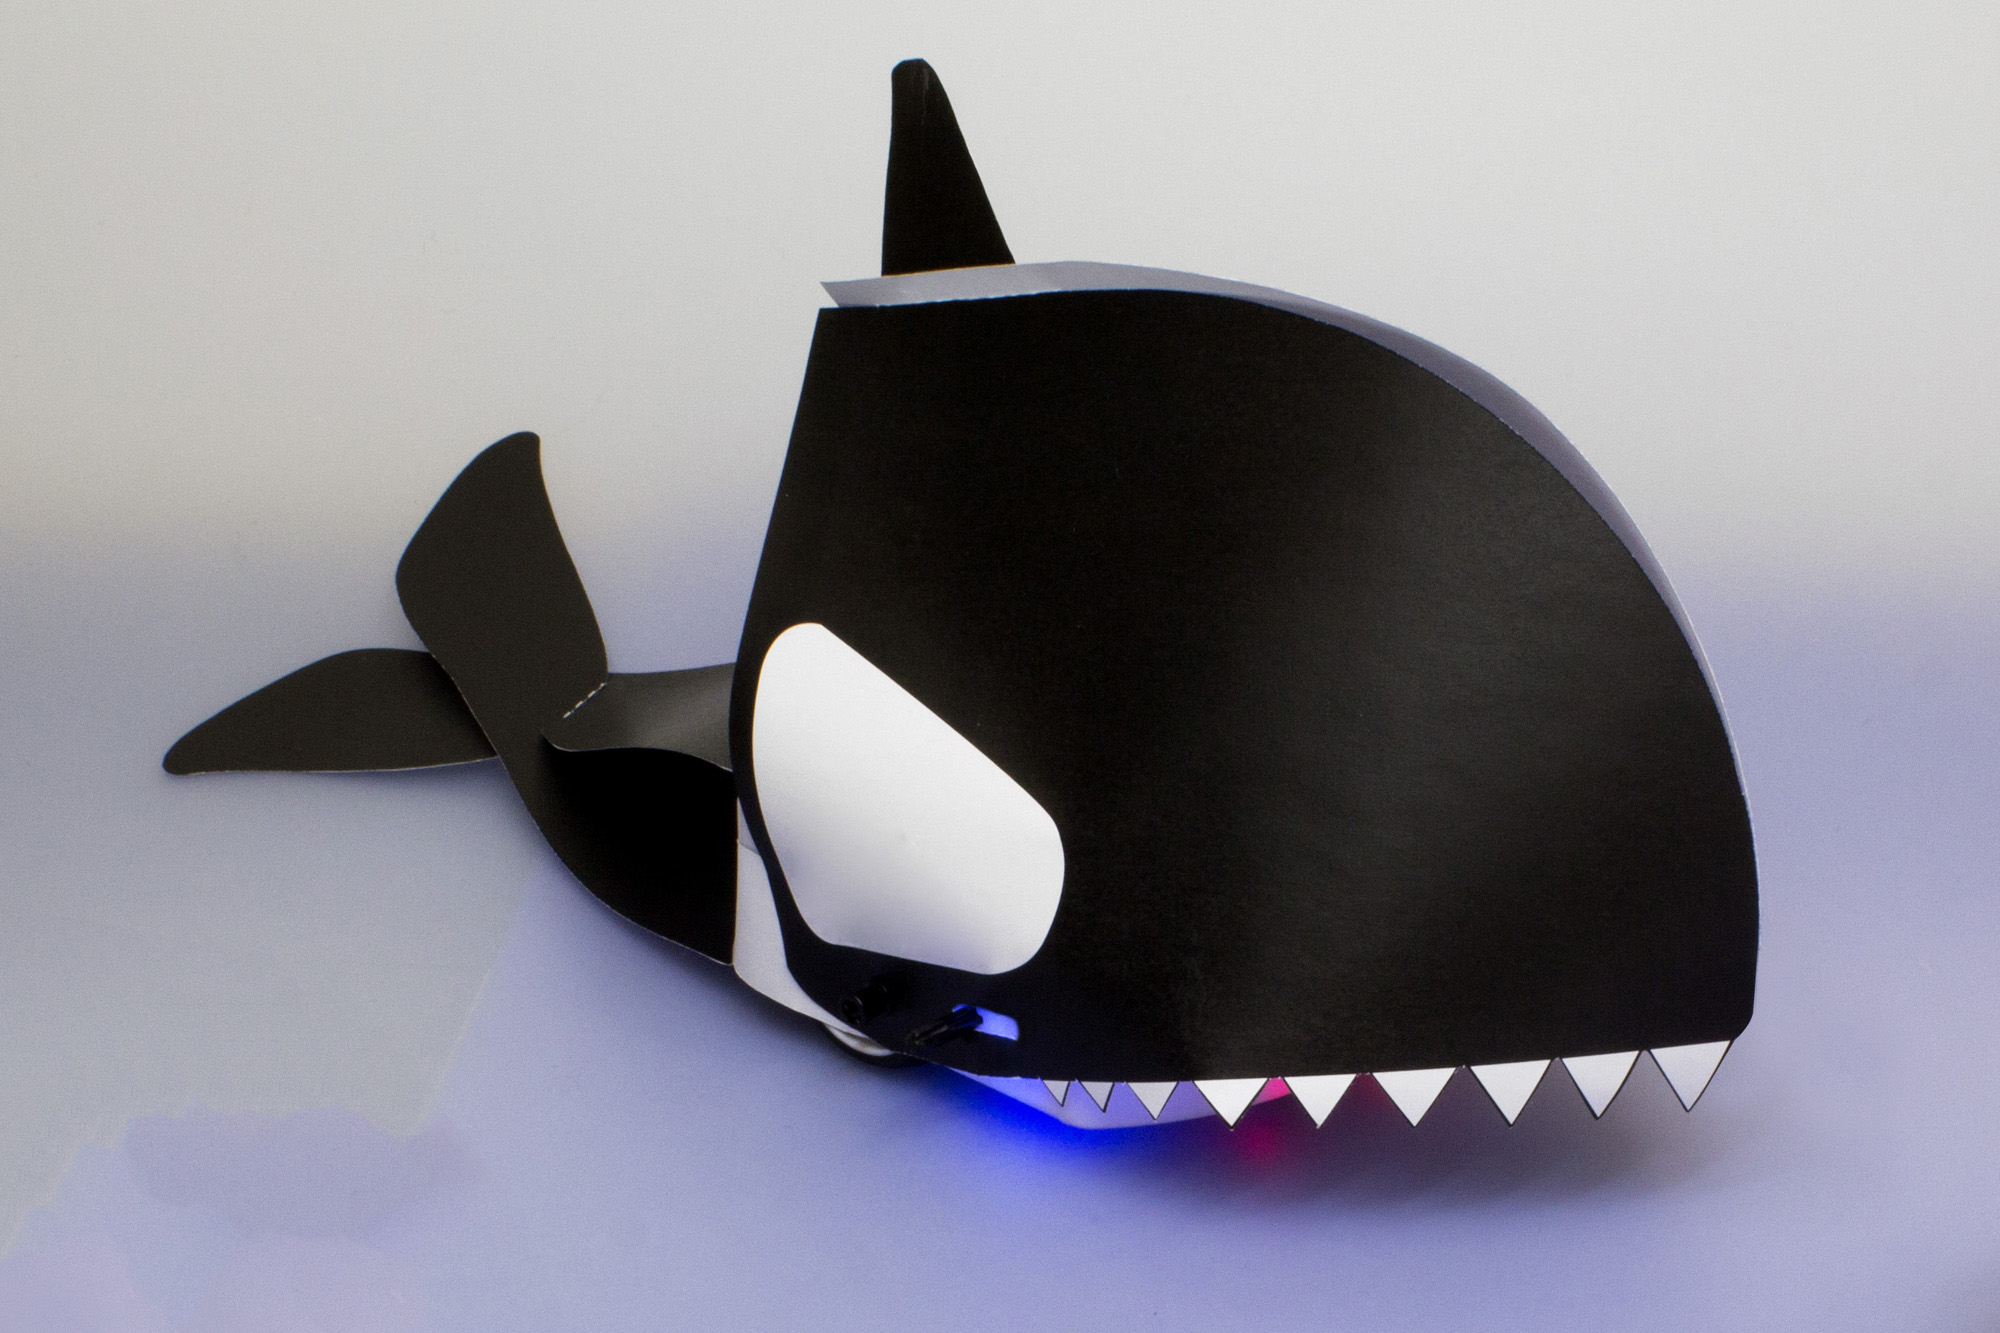
\includegraphics[width=.49\columnwidth]{figures/orca}\hfill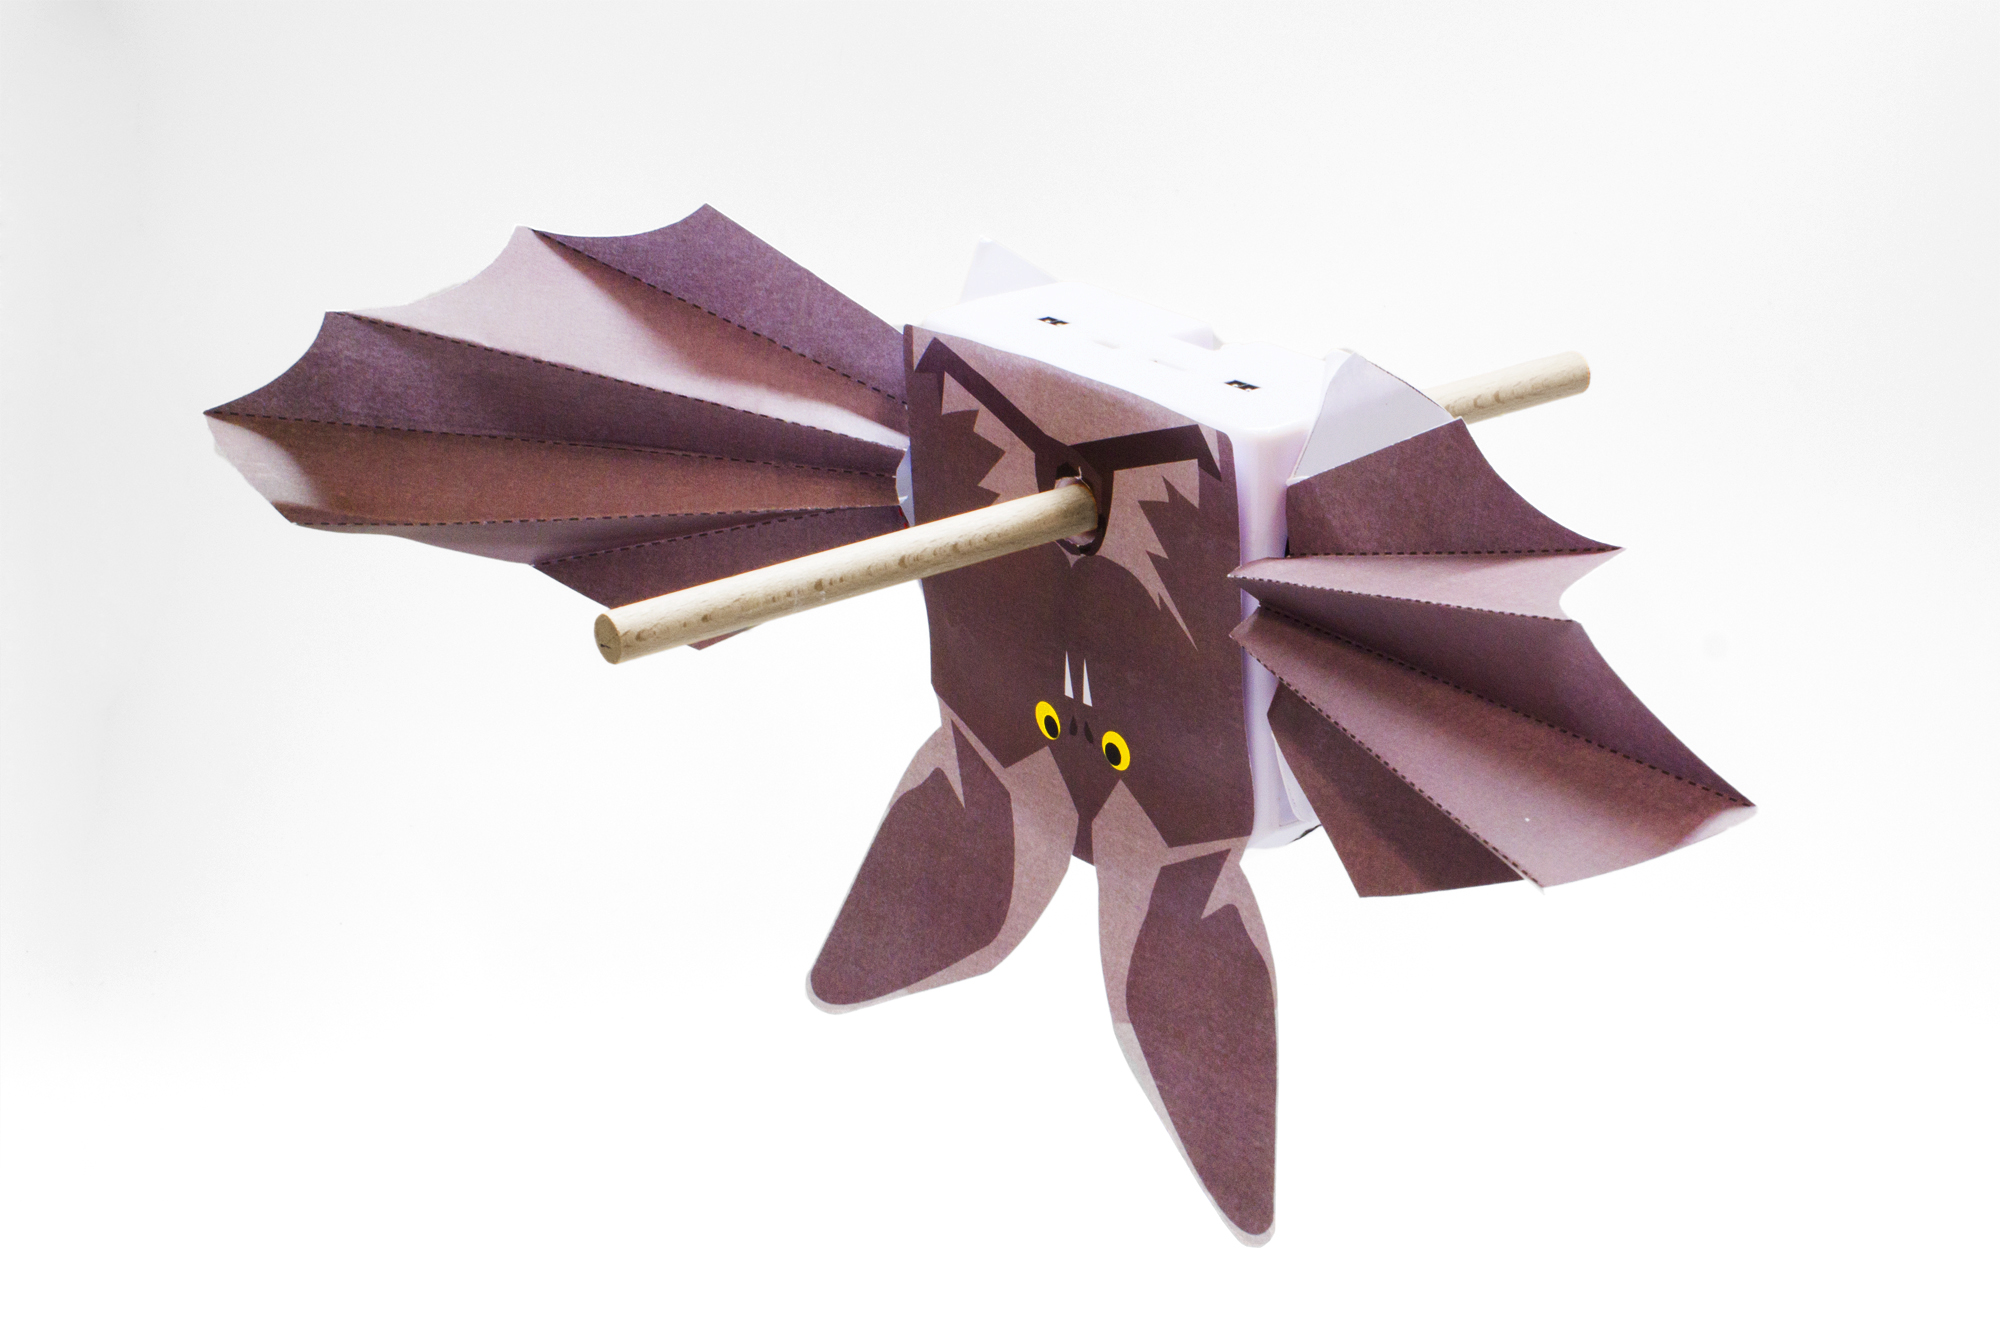
\includegraphics[width=.49\columnwidth]{figures/bat}
\vskip .5em
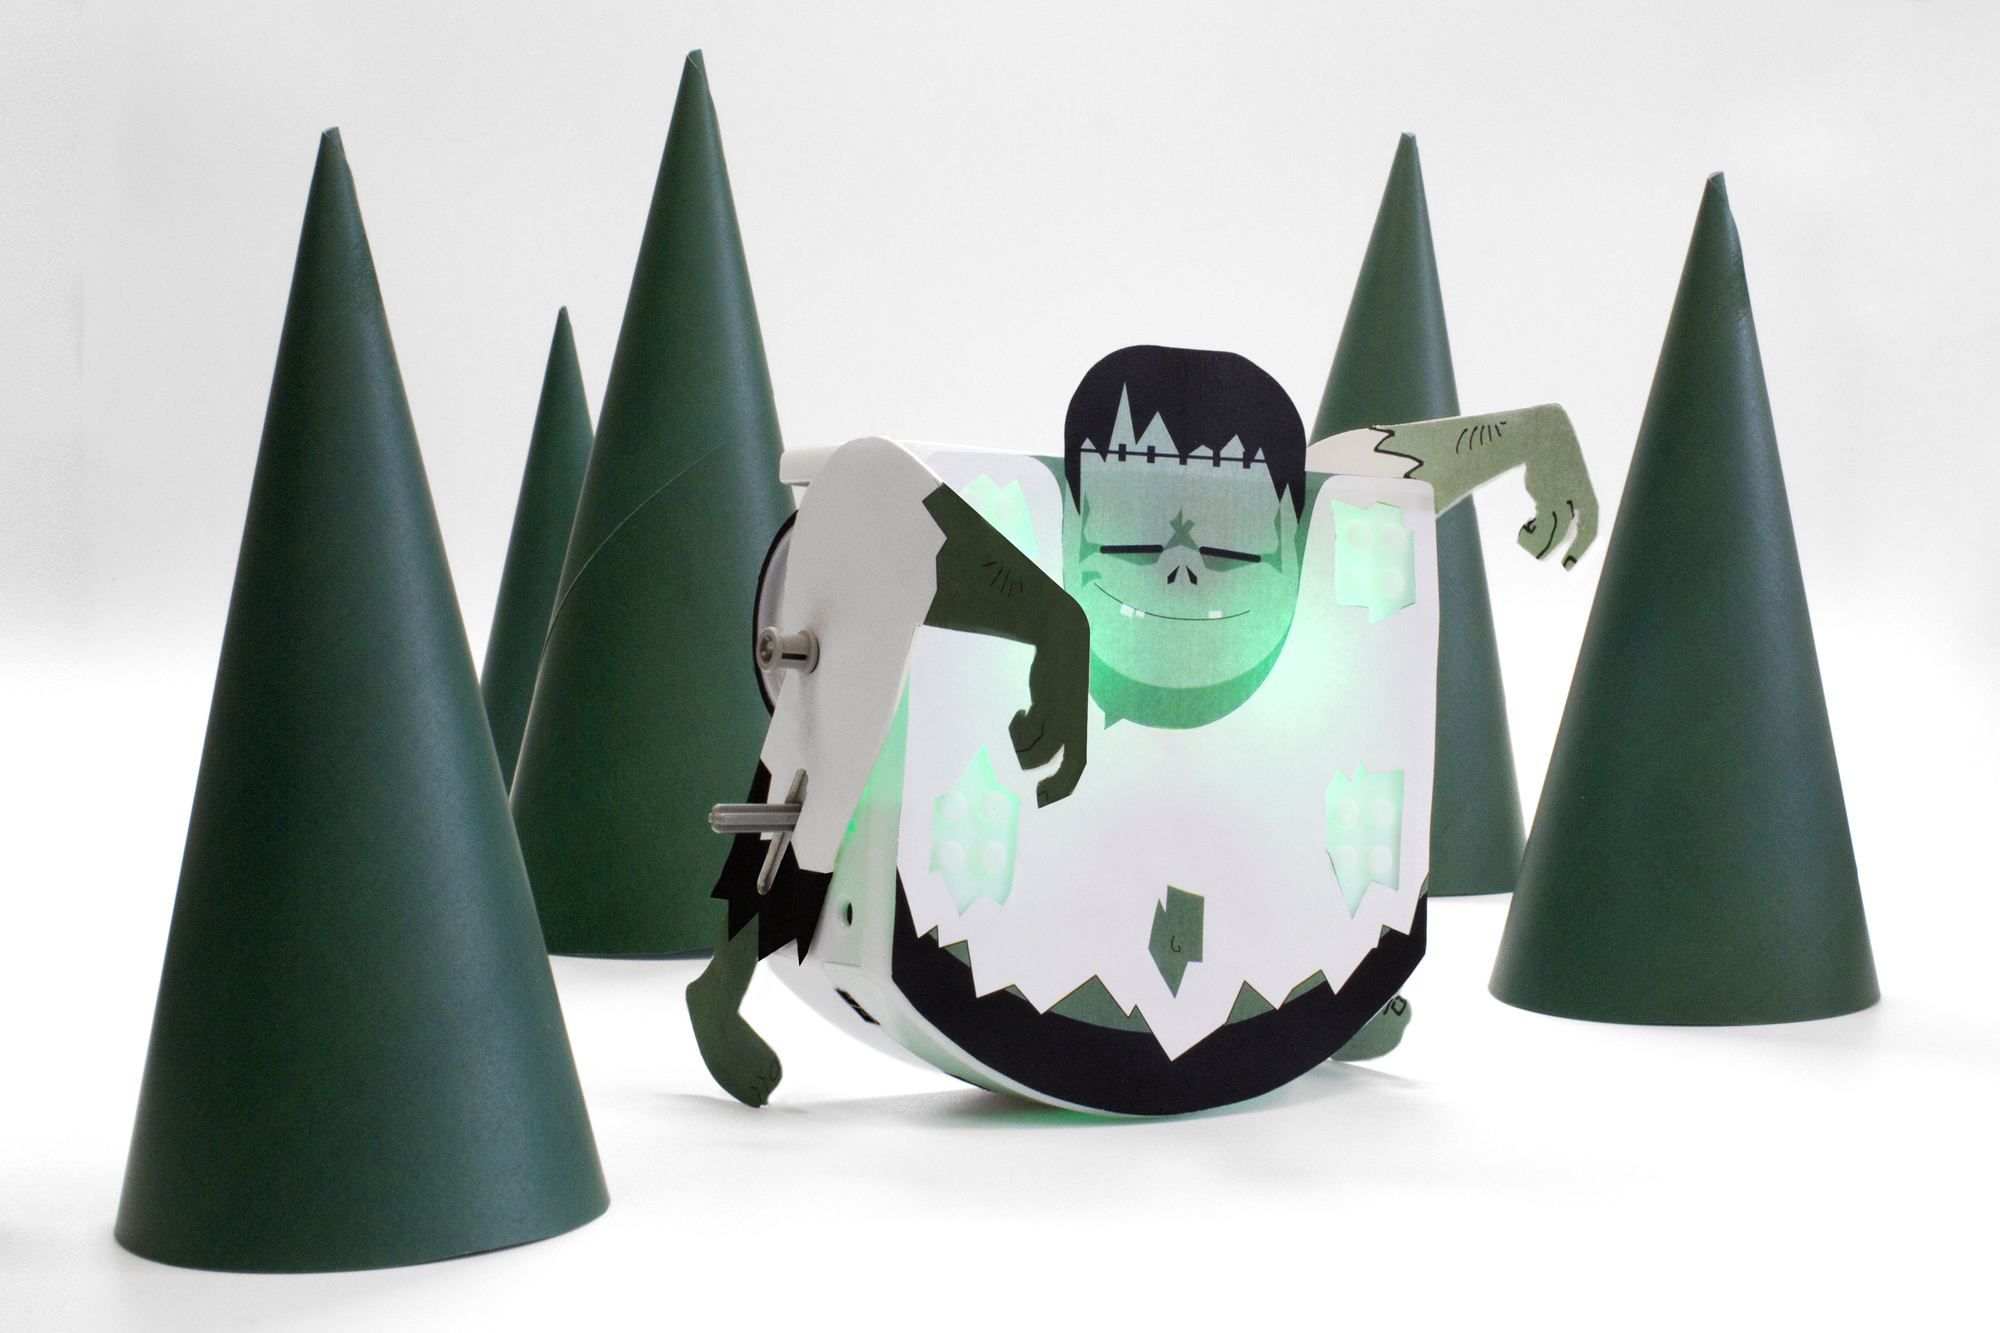
\includegraphics[width=.49\columnwidth]{figures/zombie}\hfill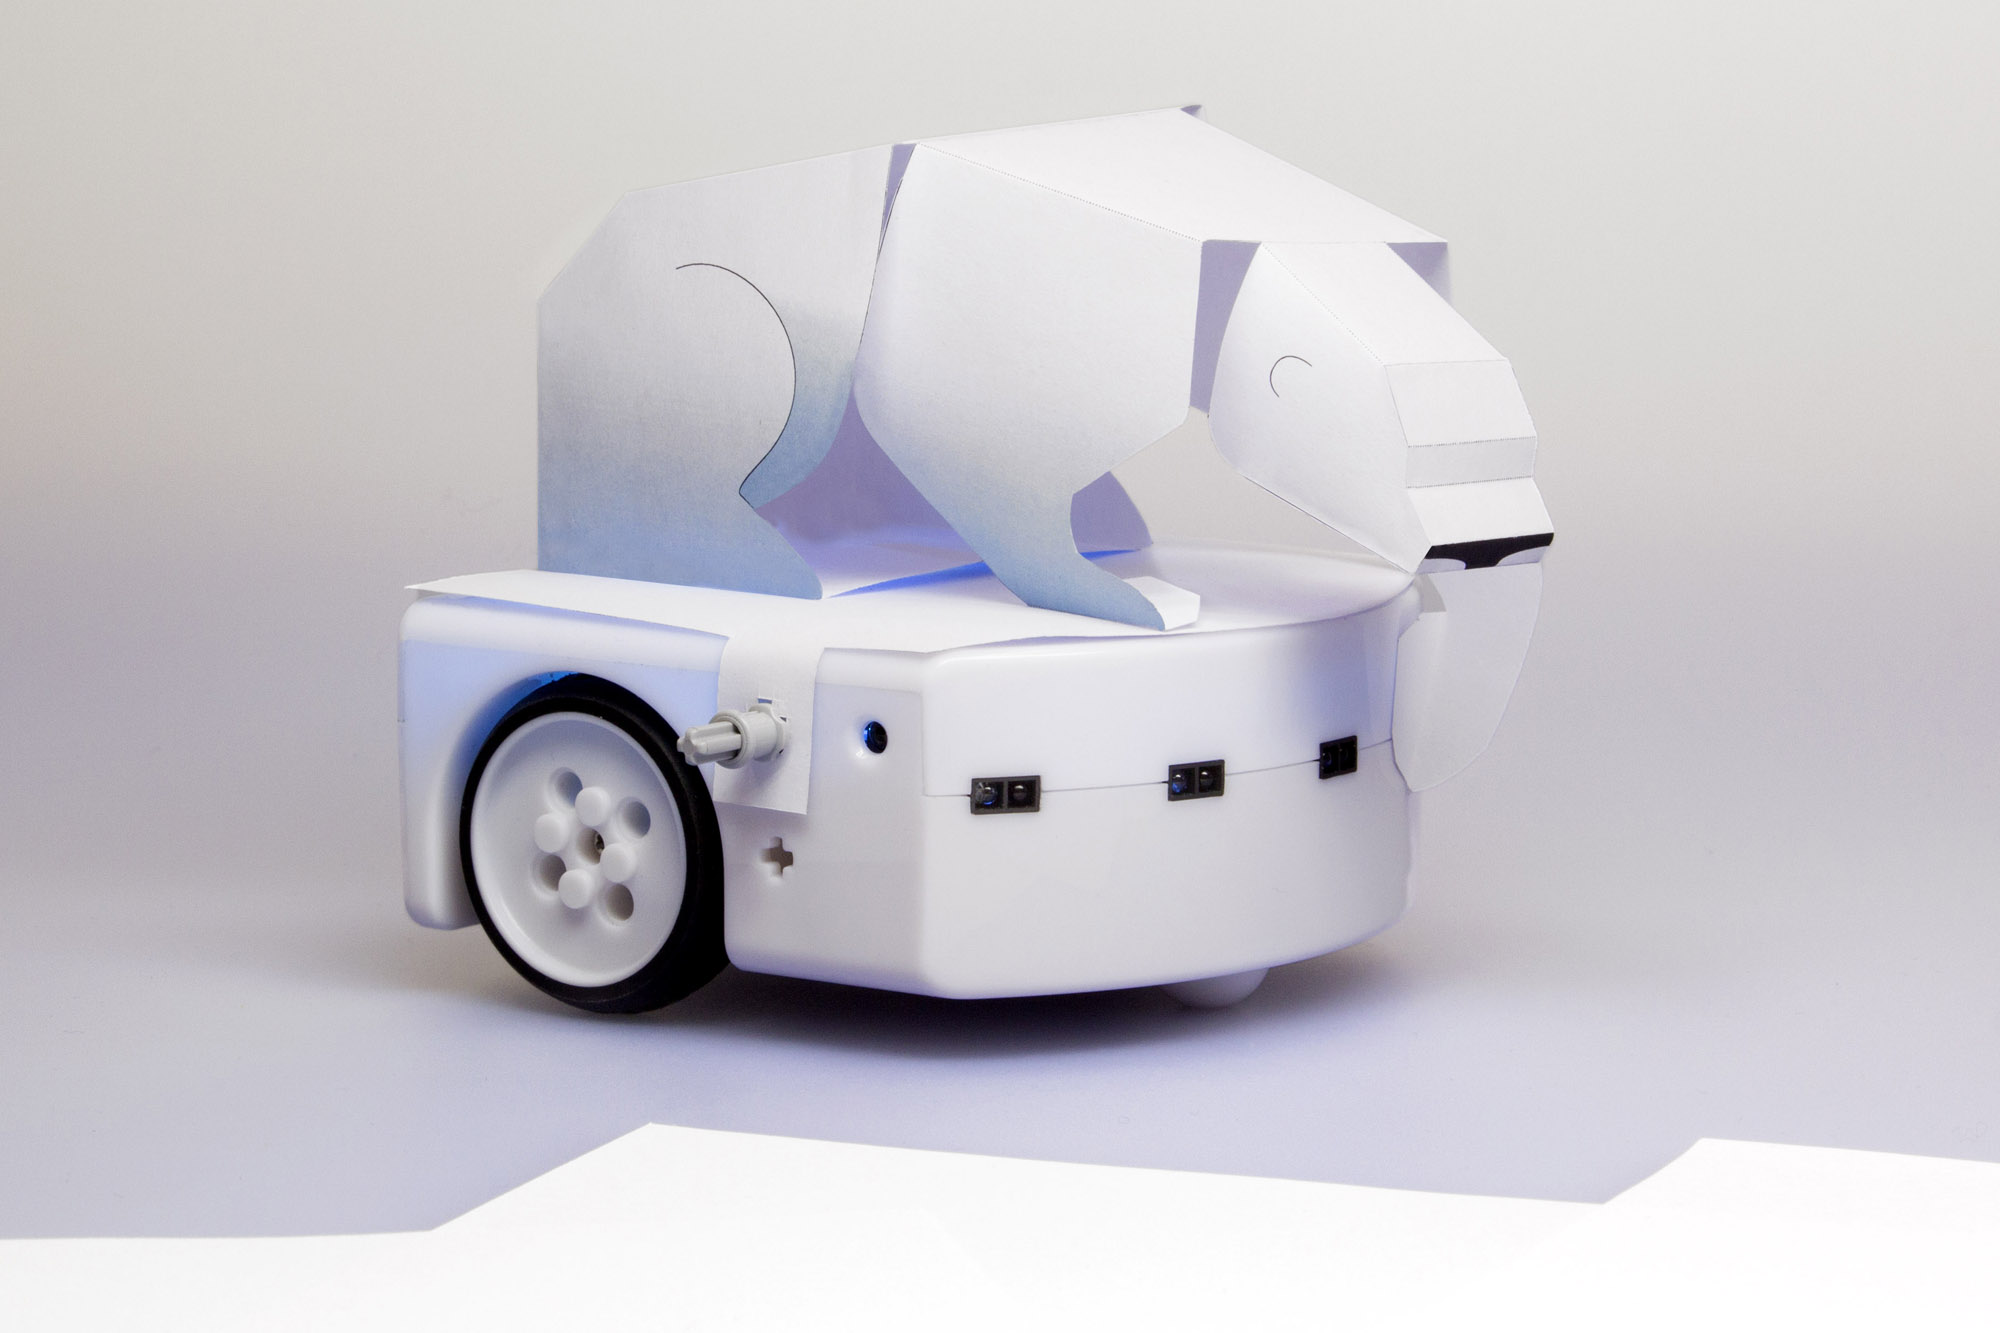
\includegraphics[width=.49\columnwidth]{figures/ours}
\vskip .5em
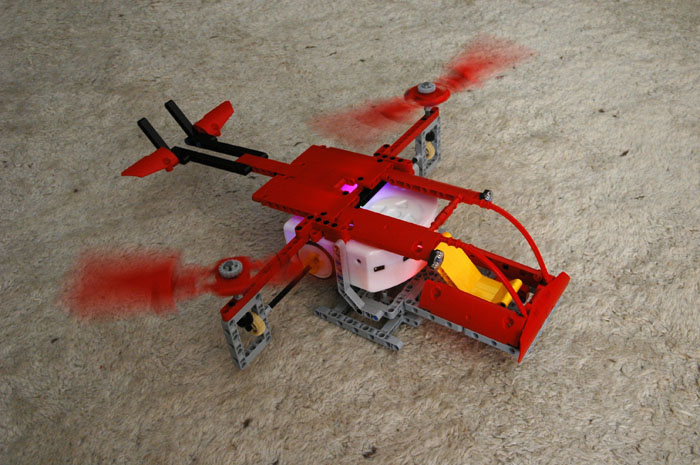
\includegraphics[width=.49\columnwidth]{figures/moving-heli}\hfill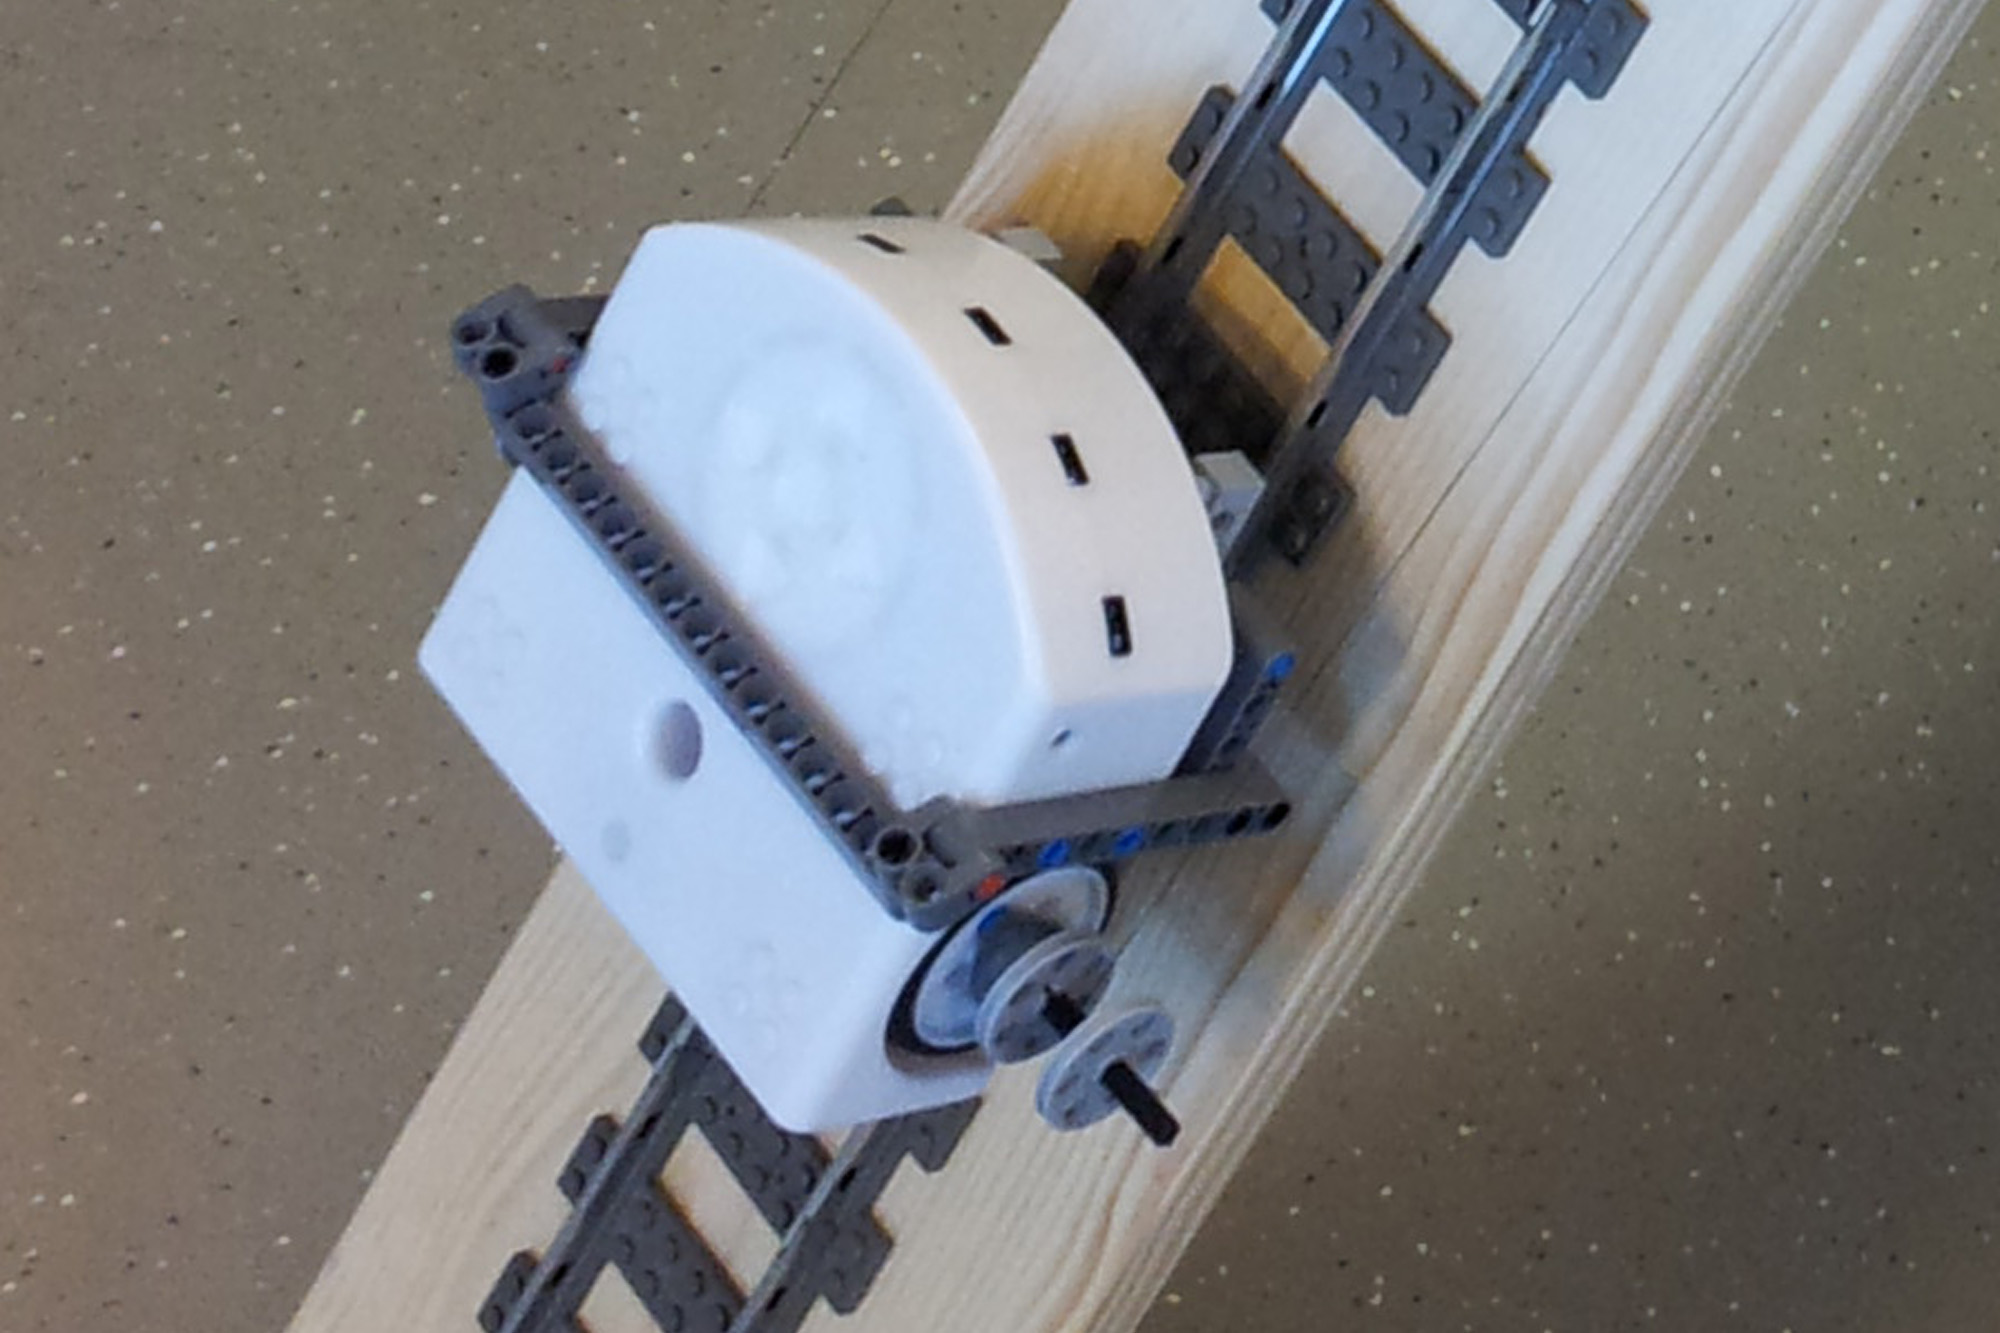
\includegraphics[width=.49\columnwidth]{figures/funi}
\vskip .5em
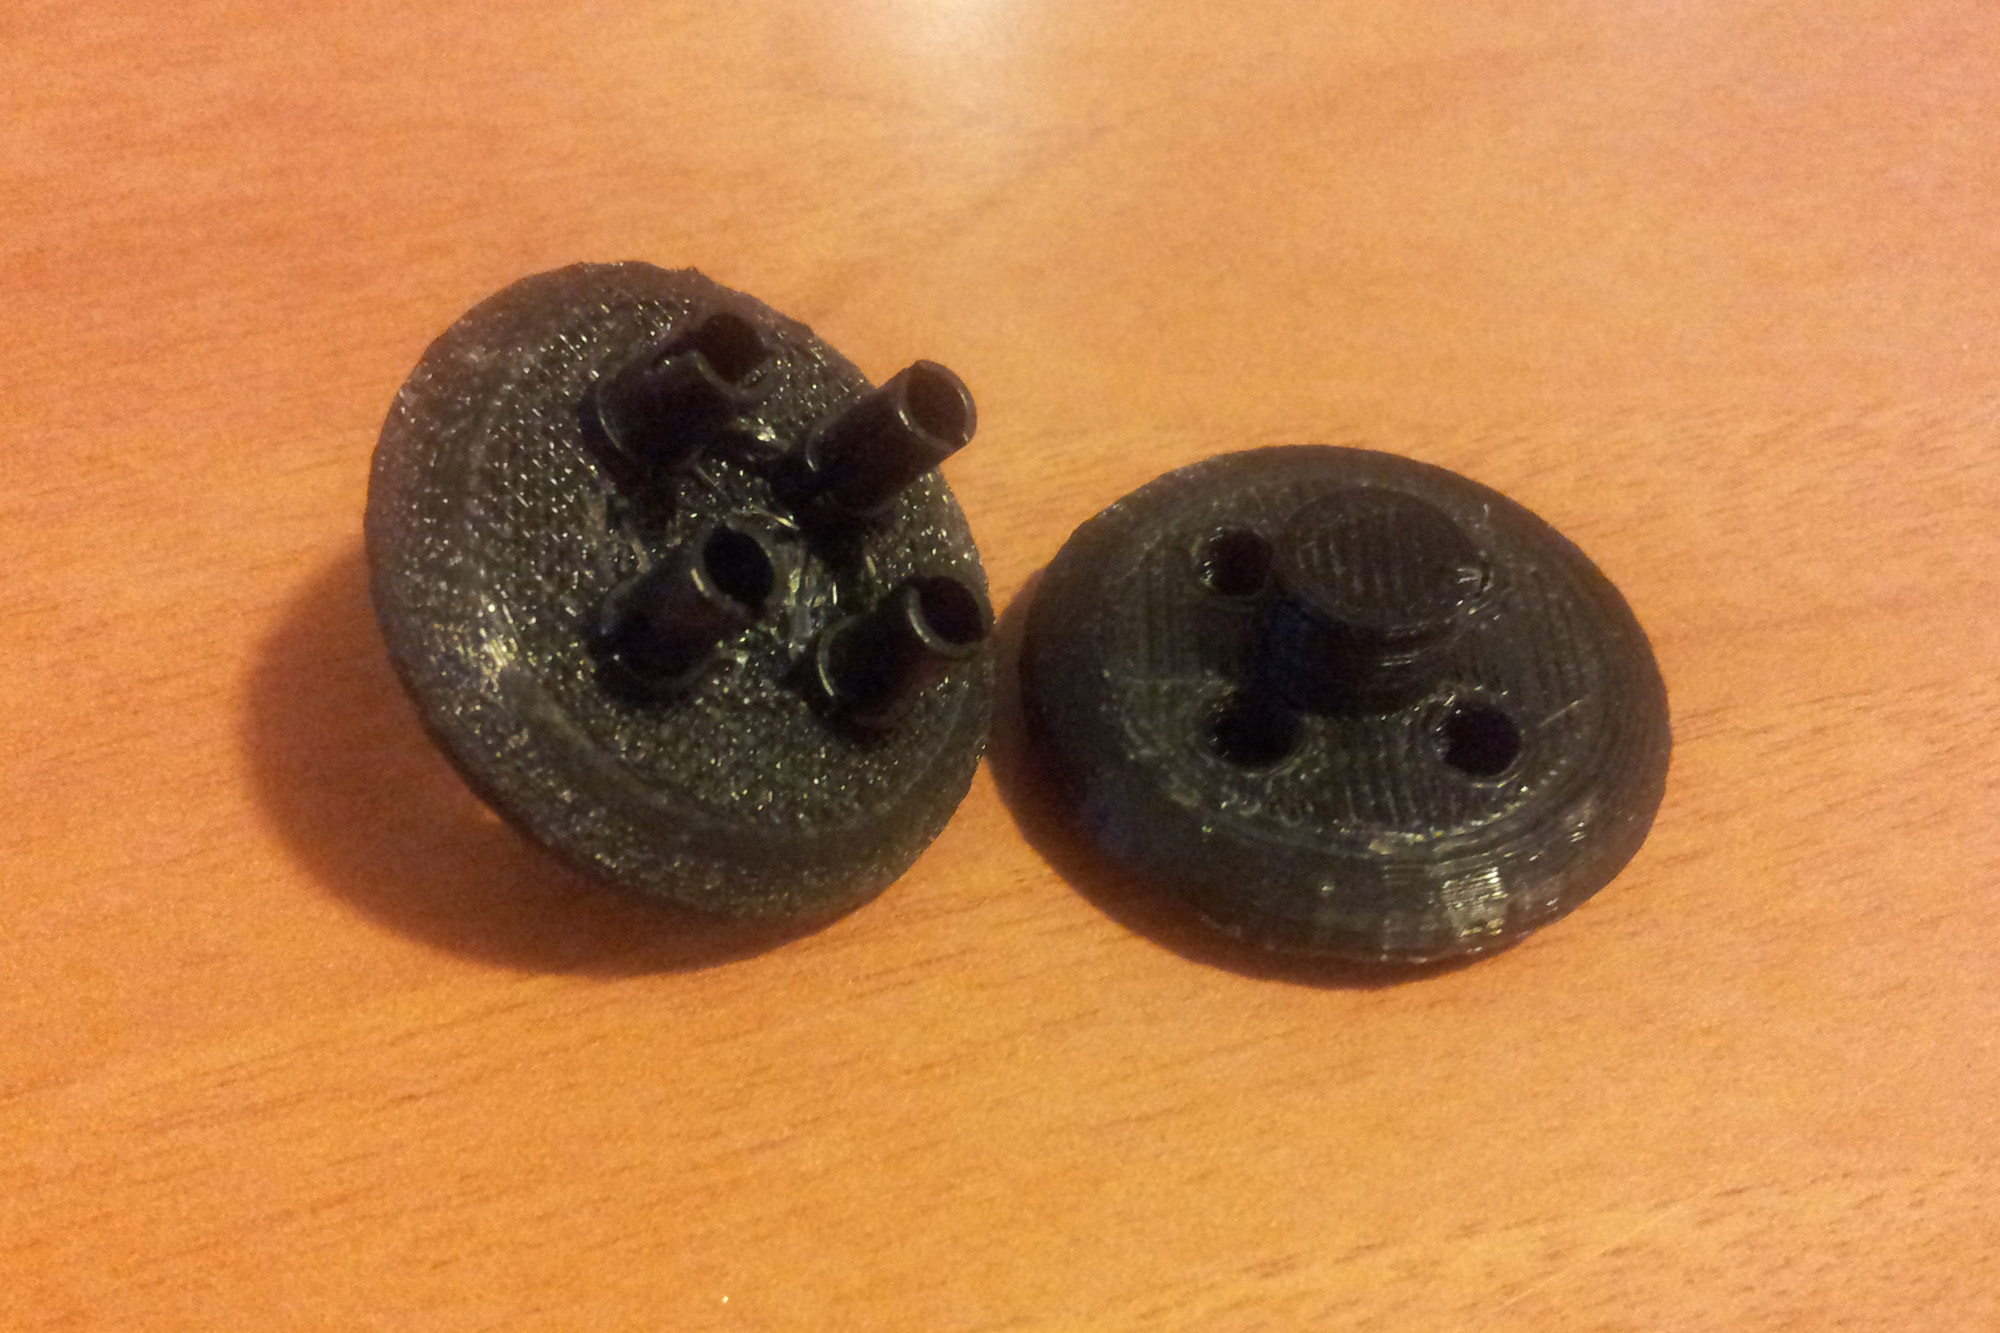
\includegraphics[width=.49\columnwidth]{figures/both_half_winder}\hfill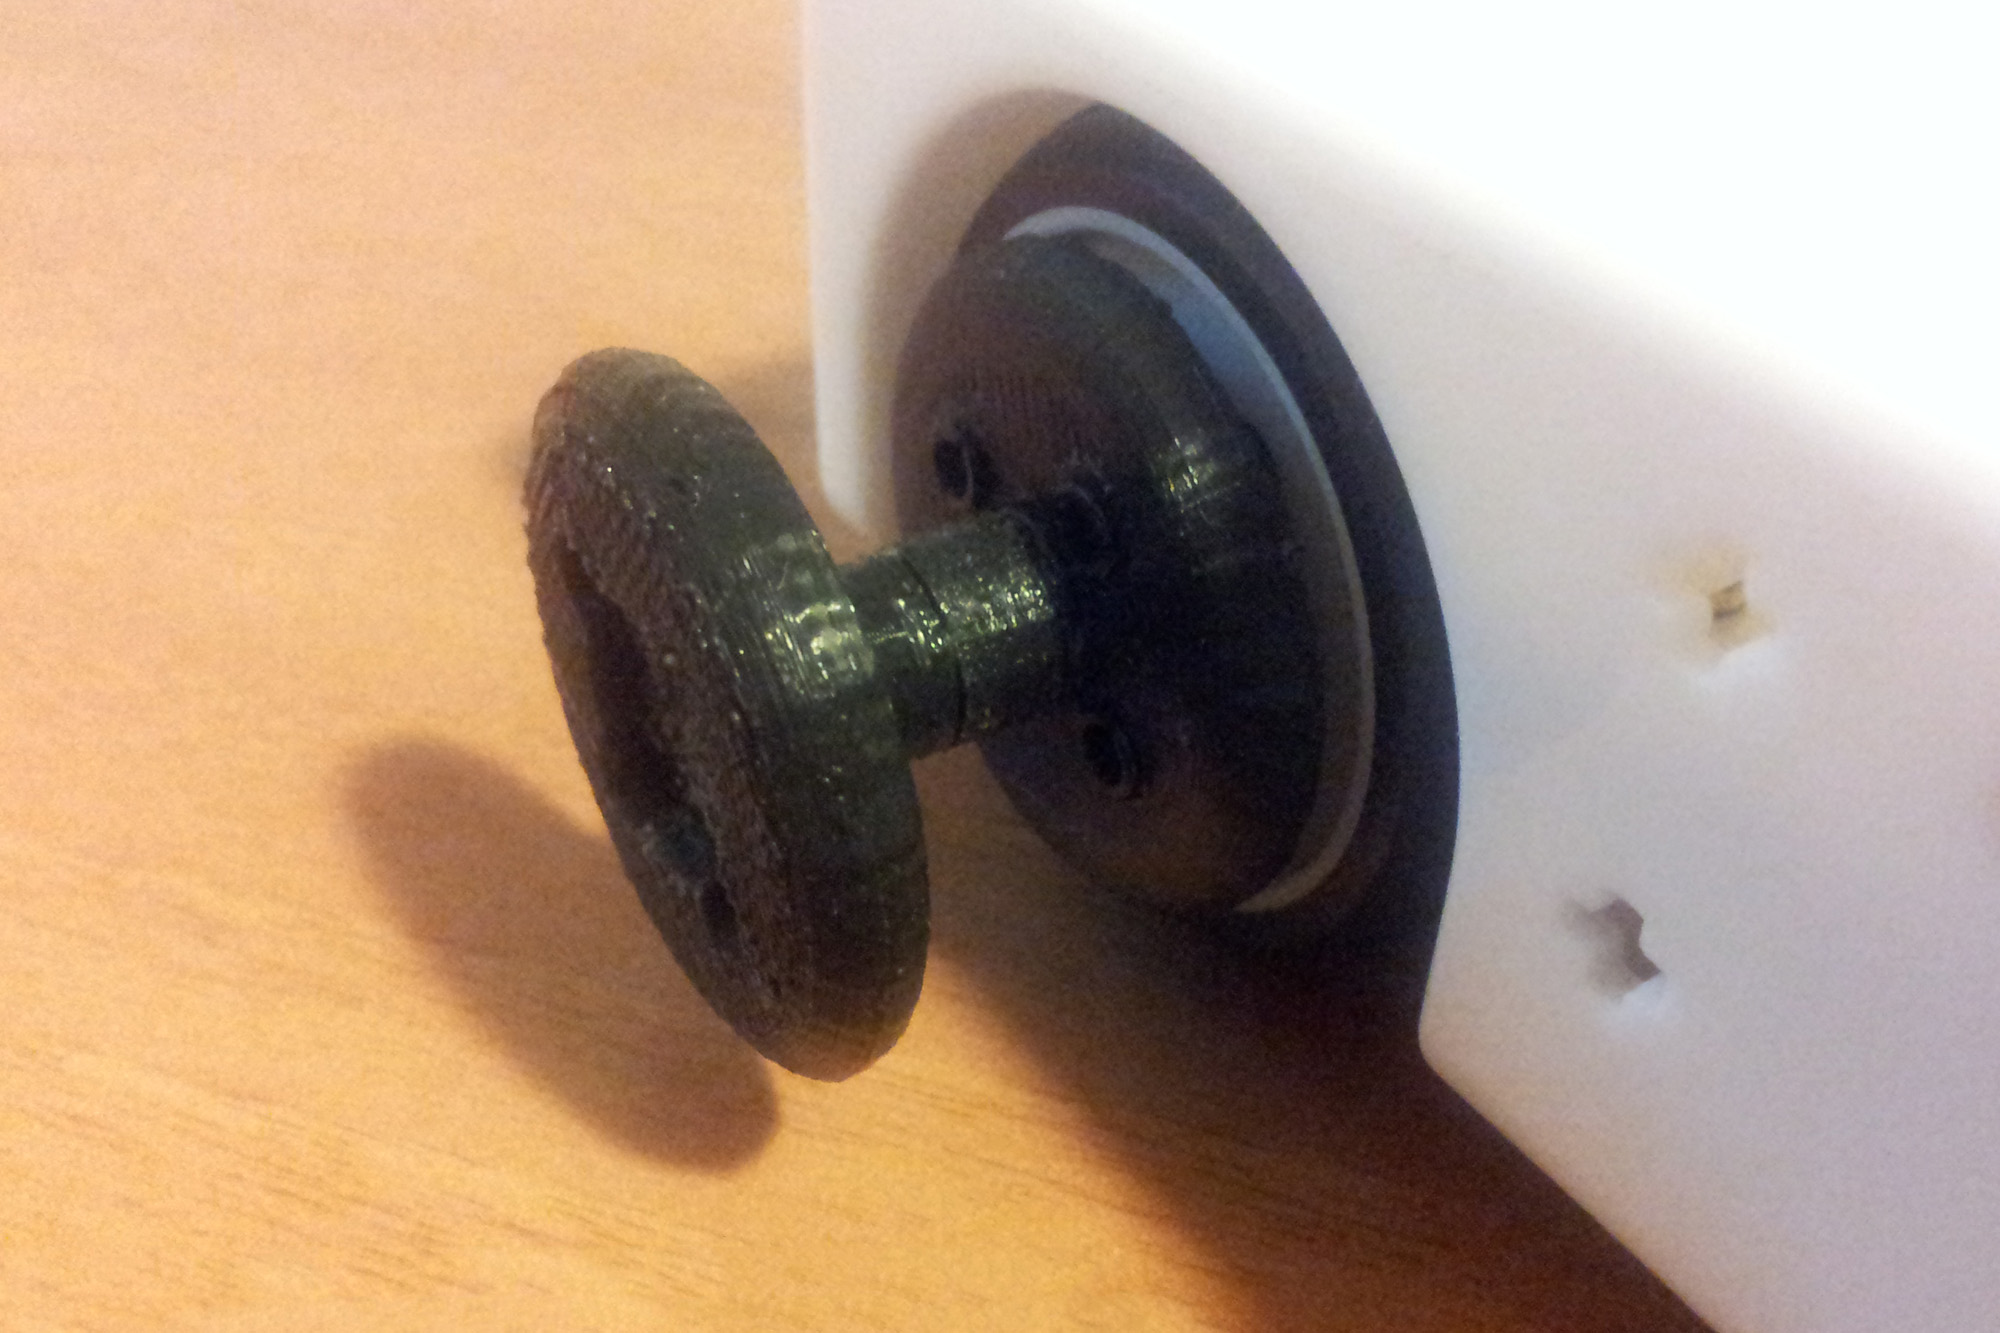
\includegraphics[width=.49\columnwidth]{figures/winder_on_thymio2}
\vskip .5em
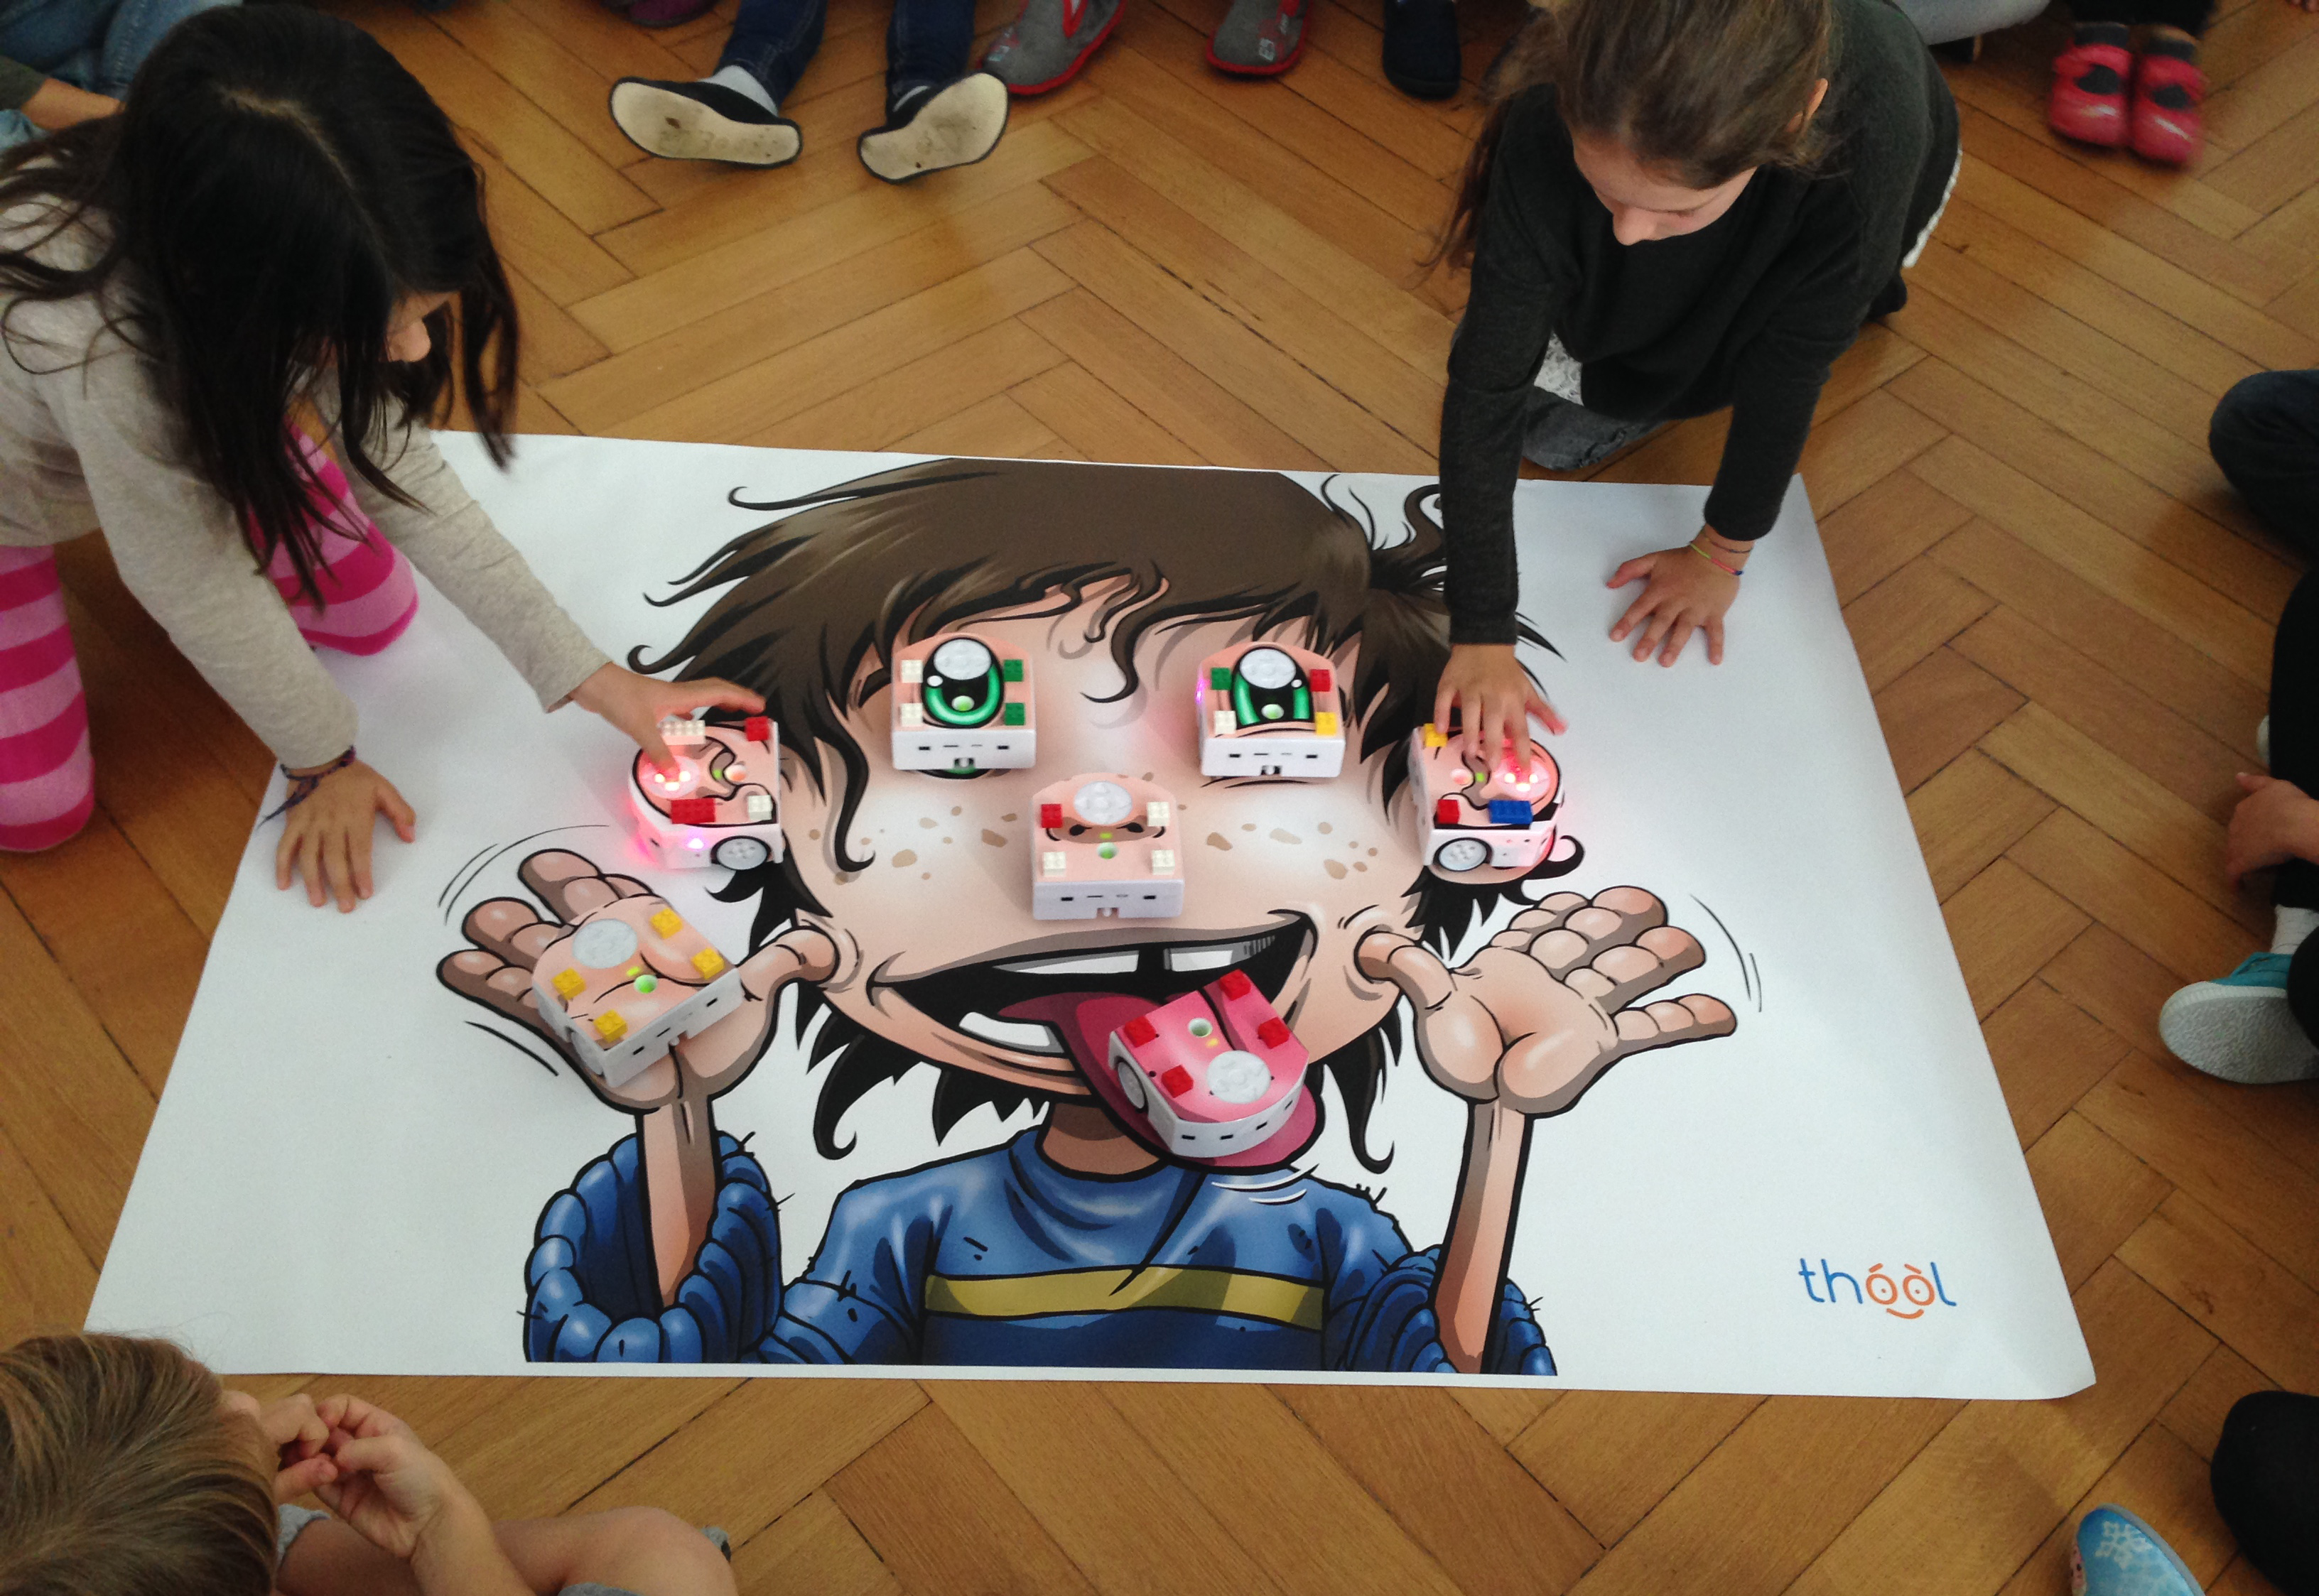
\includegraphics[width=\columnwidth]{figures/5senses}
\caption{Examples of extensions of the Thymio basic robot with paper or cardboard body extensions (top four images), using LEGO\textsuperscript{\textregistered} structural extensions (third row), using 3D-printed extensions (fourth row) or using a printed environment (bottom).}
\label{fig:example-construction}
\end{figure}



\subsection{Fast access to robotics behaviors}
\label{sec:behaviors}

Many existing robots need to be built or configured before having the first operational behavior. 
This is a barrier for many users and we wanted to avoid it carefully, having a robot able to show interesting behaviors right out of the box.
Therefore Thymio provides 6 different basic behaviors (see table \ref{tbl:basic-behaviors}), which are accessible as soon as the robot is started and are stored in flash permanently, also if the Thymio is reprogrammed by the user.
These basic behaviors allow people starting Thymio to immediately interact with it, while illustrating the many possibilities of the robot.
The behaviors are interactive and oriented towards the user. % SM: FIXME: not clear what "oriented towards the user" means
For each behavior, the robot's body has a different color, allowing the user to easily recognize it.
The user can navigate between the colors with the buttons and select the behavior she/he wants to use.
Basic behaviors can be exploited in a construction to create reactivity without the use of programming (see Figure~\ref{fig:example-construction}, the top four paper creations can be used with basic behaviors).

\begin{table}
\begin{tabularx}{\columnwidth}{@{}llll@{}}
\toprule
mode & color & sensors & behavior \\
\midrule
friendly & green & infrared (IR) & follows an object at distance \\
explorer & yellow & IR & moves avoiding obstacles \\
fearful & red & acc., IR & flees, notifies shocks and falls \\
investigator & cyan & IR & follows a black track \\
obedient & magenta & buttons, IR & follows moving orders \\
attentive & blue & mic. & moves following sound \\
\bottomrule
\end{tabularx}
\caption{The different basic behaviors with sensors used.}
\label{tbl:basic-behaviors}
\end{table}


\subsection{Programming}
\label{sec:aseba}

Thymio runs the Aseba open-source programming environment~\cite{aseba}.
Aseba is designed to enable novices to program robots easily.
On the robot side, it provides a lightweight virtual machine that runs on microcontrollers like the PIC24F.
A virtual machine allows instantaneous upload and safe execution of code.
On the desktop side, Aseba provides an IDE which allows to program in a purely graphical mode (called VPL, see Figure~\ref{fig:vpl}), or using a scripting language (see Figure~\ref{fig:aseba-studio}) or in a mixed way, assembling code in a graphical way using the blockly environment\footnote{\url{https://developers.google.com/blockly/}} (see Figure~\ref{fig:blockly}).
This allows the IDE to match with the multi-age goal described in section~\ref{sec:multi}.


%The Aseba scripting language is a simple, imperative, Matlab-like language providing integers and arrays of integers as data types.
%Common logical and mathematical operations are available as operators, and additional mathematical functions such as trigonometric ones are available as native functions.
%These are functions implemented in native code and accessible from the virtual machine.
%In Aseba, code blocks are associated to events, simplifying the writing of real-time behaviors.
%Events are triggered by the robot's sensors or actuators.
%The value of the sensors and actuators are available through pre-defined variables and native functions, which are robot-dependent and enumerated dynamically by the robot when the IDE connects.

The IDE integrates real-time feedback both graphically under VPL~\cite{Magnenat2015} and displaying variables or graphs in the text mode.
The IDE also provides a help documentation\footnote{currently English, French, and German}.
In addition, the wiki pages of the project provide tutorials on programming with Thymio and a detailed description of the programming interface.
%The latter was designed with consistency in mind: variables and functions are available in namespaces and similar features (such as the different LEDs) are accessed the same way.
%It also provides native functions for school-level mathematics such as vector operations, trigonometry, statistics and functions such as sorting and random.

%We expect the facilities that Aseba provides to allow text-based programming with reasonably young children, starting from around 10 years old, while still being interesting to older children and adults.
Aseba integrates with \textsc{ros}~\cite{quigley2009ros} through the \emph{asebaros}\footnote{\url{http://www.ros.org/wiki/asebaros}} bridge.
\textsc{Ros} is one of the most widely used software framework in robotics research, and this integration allows to run sophisticated algorithms, such as simultaneous localization and mapping, in conjunction with  Thymio.
This makes the robot suitable for university-level education.

\begin{figure}
\centering
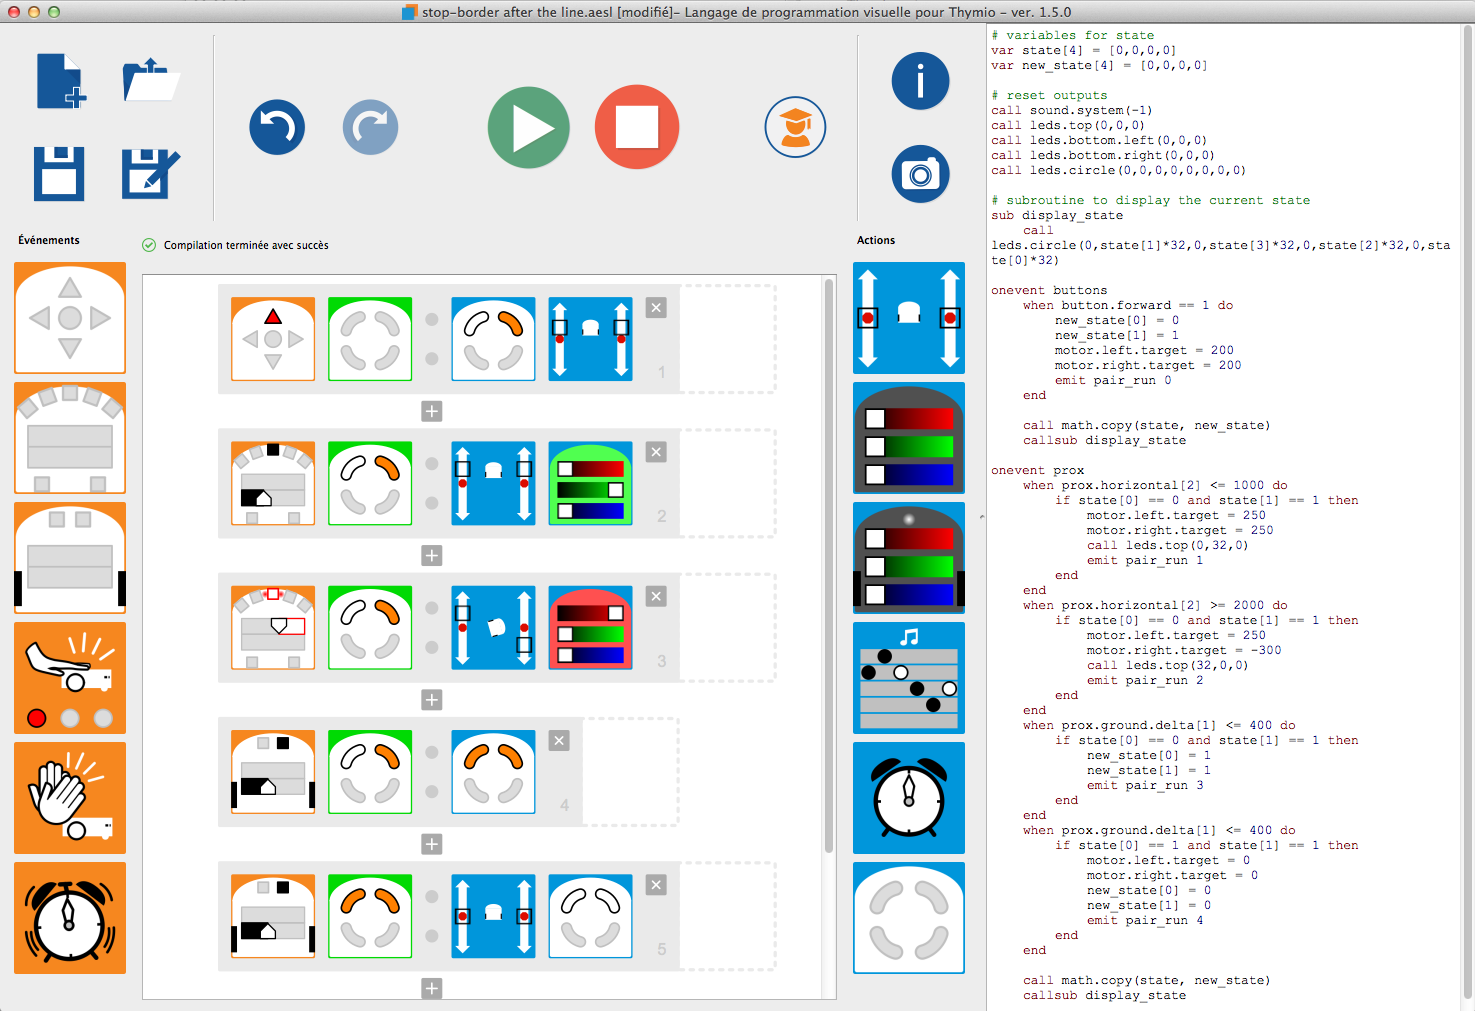
\includegraphics[width=.9\columnwidth]{figures/vpl}
\caption{The graphic programming environment VPL.}
\label{fig:vpl}
\end{figure}

\begin{figure}
\centering
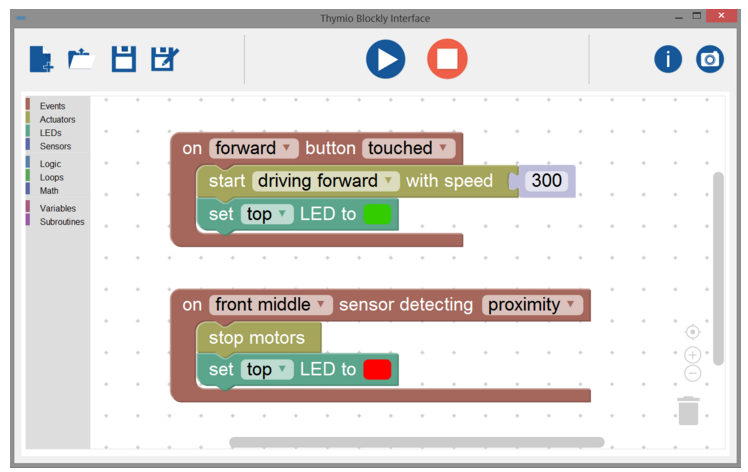
\includegraphics[width=.9\columnwidth]{figures/blockly}
\caption{The blockly programming environment.}
\label{fig:blockly}
\end{figure}

\begin{figure}
\centering
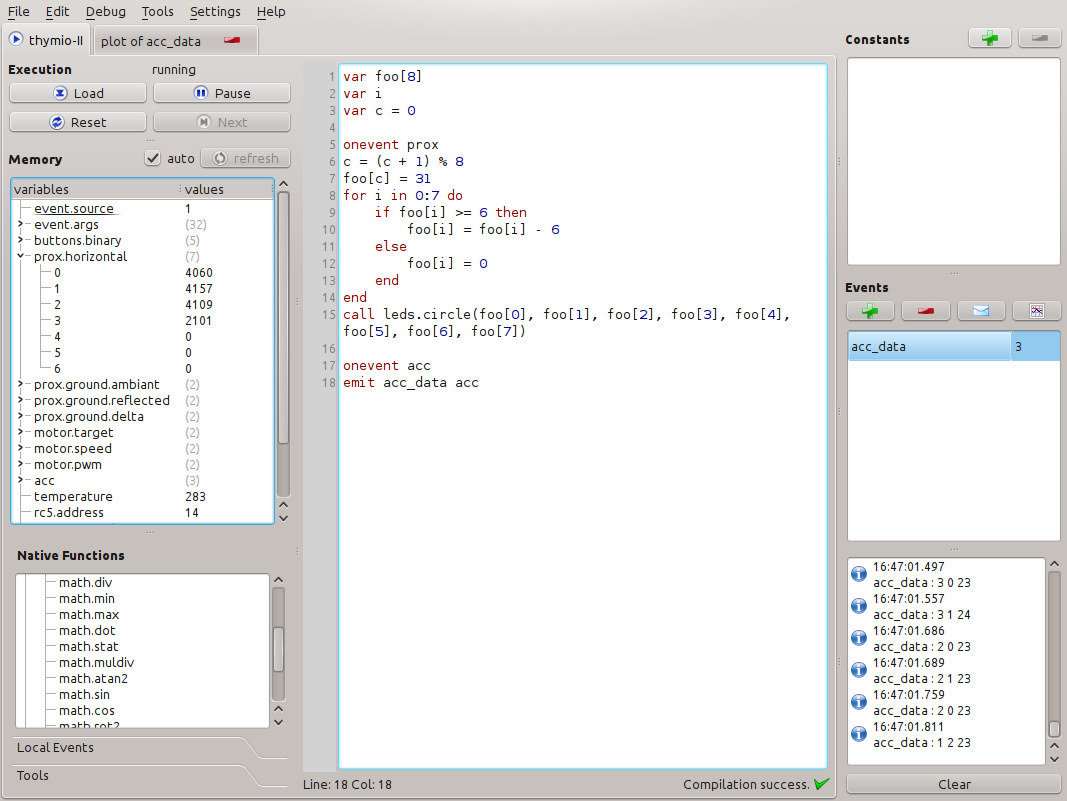
\includegraphics[width=.9\columnwidth]{figures/aseba-studio}
\caption{Aseba Studio, the integrated development environment}
\label{fig:aseba-studio}
\end{figure}

\section{Open source hardware, choices and impact}

The choice of developing a robot within an open source hardware project has an impact on the robot design and the way this device is used in the community of users. 
In this section we analyze more in detail the implications of this choice in the context of educational robotics.
We compare these implications with the result of a survey that got 35 answers from people active in various open source hardware projects based on a worldwide call for contributions. 
Among these 35 answers, 11 come from project leaders, 13 from core design team members, 8 from contributors and 3 from enthusiastic users.
54\% of these respondents are between 25 and 35 years old, 26\% between 35 and 50 years old, 9\% are less than 25 years old and 11\% are older than 50.  
67\% either work in an academic environment or are students. 
34 of the 35 answers come from male respondents.

\subsection{Motivation}

We can distinguish two levels of motivation, the institutional and the personal one.
The institution initiating a project is mainly looking for recognition and/or money. 
Our group has a good experience in disseminating robotic hardware with the Khepera~\cite{MonFraIen93} and e-puck~\cite{mondada2009puck} robots.
Khepera was disseminated with a proprietary strategy, e-puck with an open source hardware one.
Both were targeting similar users and have been sold in similar quantities.
What we can observe after more than 10 years is that Khepera generated many royalties for the university, but less relative academic visibility than e-puck (see Figure~\ref{fig:khepuck}) .
The e-puck robot, being open hardware and with an image better linked to the university, generated no income for the university but much more visibility in respect to his diffusion.
Khepera was more linked with the name of the company producing it, the e-puck robot was nearly not linked with the producer when mentioned in the literature.
In the case of Thymio, developed in a research project, the institutional motivation was to get visibility more than money. 
Therefore, based on the past experience, the open source hardware strategy seemed more adapted.

\begin{figure}
\centering
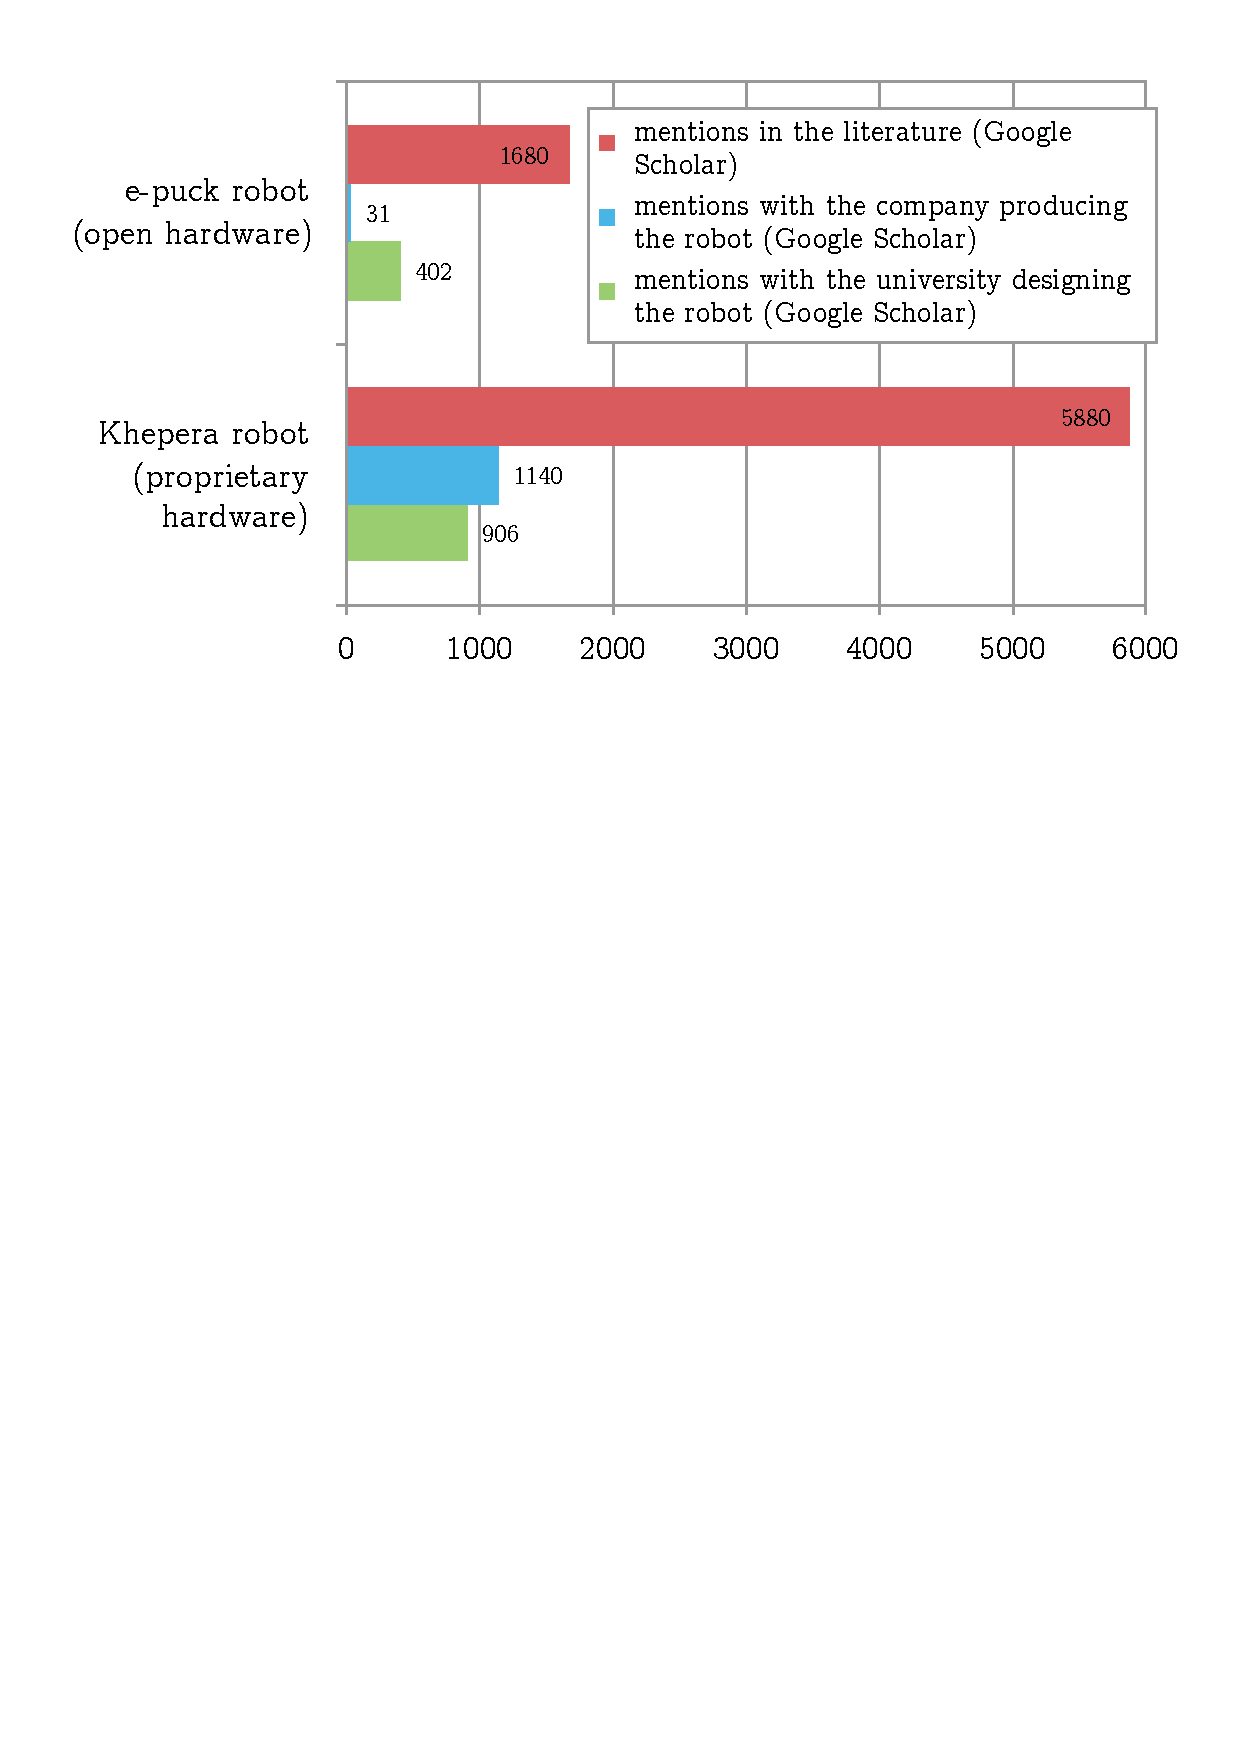
\includegraphics[width=\columnwidth]{figures/others_robots}
\caption{Comparison between mentions in the literature, mention of the manufacturer and citation of the reference paper for two robots disseminated by our lab in the past. It appears that the Khepera robot, distributed with a proprietary strategy, was more linked to the company producing it than the original designers. This is the opposite for the e-puck robot, distributed with an open source license.}
\label{fig:khepuck}
\end{figure}

The personal motivation to participate to such a project is very different than the institutional one. 
When asked about their personal motivation, the people participating to the survey give as main motivation a link to their professional activity and to the specific project, followed by a more general motivation by the nature of the project and finally by the engineering practice (see Figure~\ref{fig:motivation}). 
The more abstract goal of improving our society is mentioned only by few respondents.

\begin{figure}
\centering
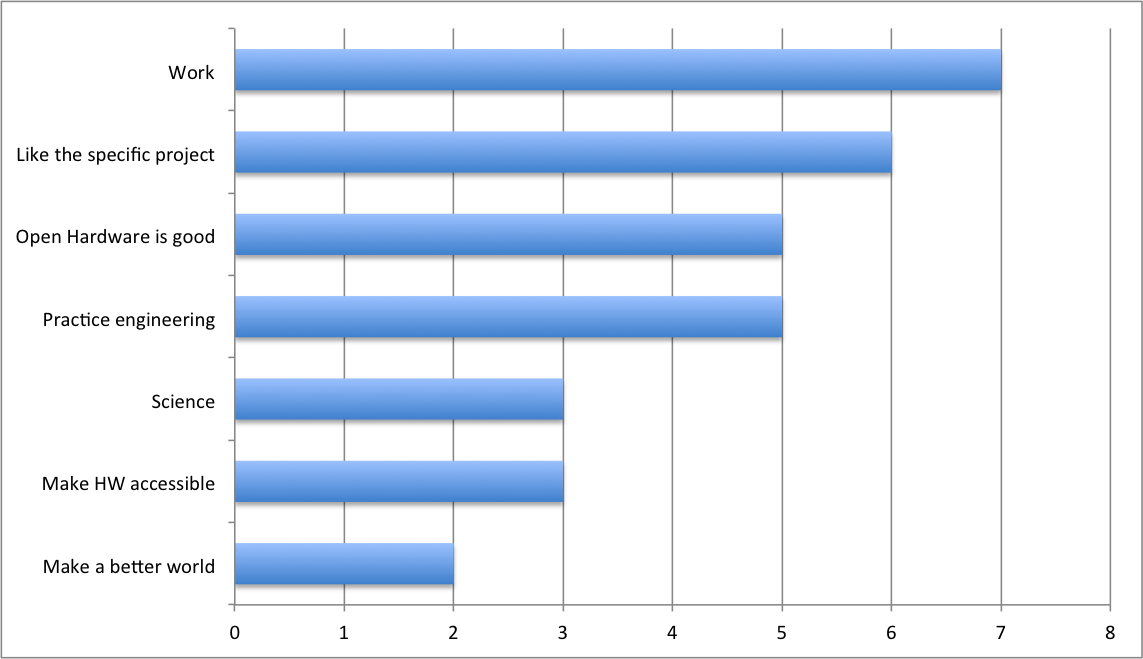
\includegraphics[width=\columnwidth]{figures/motivation}
\caption{Motivation of the people participating to the survey.}
\label{fig:motivation}
\end{figure}

In the Thymio project, most engineering contributors were hired for a research project developing the robot. 
Industrial designers also contributed as part of an institutional project.
Therefore the link with the professional activity and the particular project is evident.
On another side, the motivation of contributing to society is much stronger in our team, as developing a robot targeting education has a strong societal component.
Moreover this project has a strong scientific motivation, with several ongoing studies on the acceptance by teachers and the impact on children.
Also this motivation is therefore stronger in our team.
Although this seems a minor issue, sharing a strong fundamental motivation such as education or scientific achievements, is a key element for a strong community~\cite{Stahlbrost2011}, especially if interdisciplinary like ours.

It is also interesting to look at what people expect as benefits in participating in such a project (see Figure~\ref{fig:getout}).
Most of the answers mention impact, networking and learning. 
In these answers we can observe both a technological component in getting better results and impact, and a human-relations component that is not in the basic definition of open hardware but results from the community created around the project. 
People expect to work with other people to achieve more together, to create a network of competences or users, to learn through new experience and contacts. 

In the Thymio project we had similar expectations. 
Working together with several partners was for everybody a win-win situation, and creating a community of users was the only solution to allow the development of high quality accessories and educational material.
A wiki\footnote{http://www.thymio.org} has been established as meeting point for the learners, the robot developers, and the teachers.
It introduces the robot, explains the basic behaviors, gives access to the programming environment and its documentation, and provides code samples and examples of constructions.
The wiki is open for editing by anyone, and although we initially provided most of the material, the other members of the community have started to contribute.
One of the most important contributions to the wiki, in term of effort, has been its translation into four languages.

In addition to those elements, in our project we expected another important benefit from open hardware in term of image: we wanted a match between the non-profit nature of the project and the non-profit nature of education in general. 

\begin{figure}
\centering
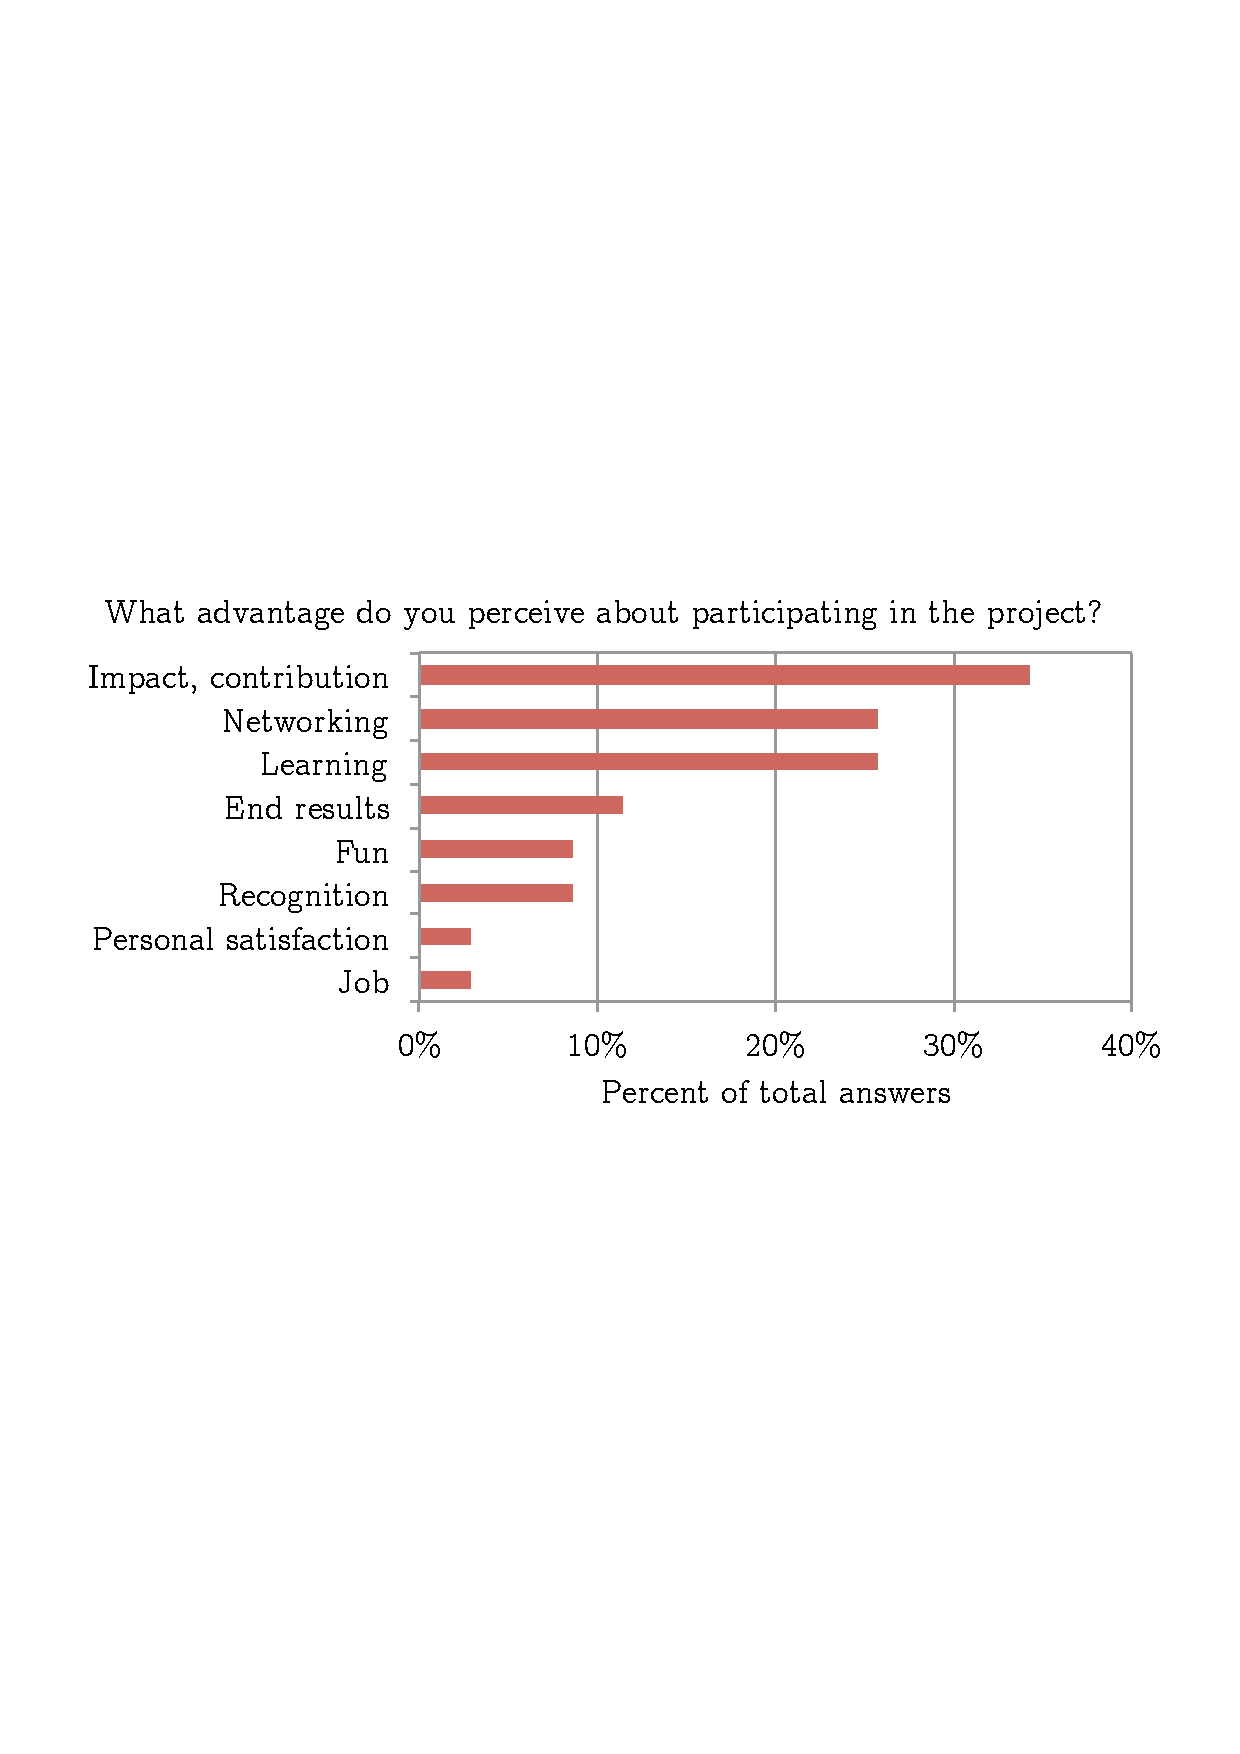
\includegraphics[width=\columnwidth]{figures/advantages}
\caption{Advantages that people participating to the survey perceive by contributing to an open source hardware project.}
\label{fig:getout}
\end{figure}

\subsection{License of project and license of tools}

When starting an open source hardware project, one of the typical questions is about which license to use when disseminating the project source files. 
We will not discuss this matter here, as it is a very common and well-covered issue. 

There is another licensing issue which is not well known and that we discovered very late in our project: the constrains of the license of the mechanical and electronic CAD tools. 
Indeed, asked about this issue, the participants to our survey seem generally not aware of the fact that CAD licenses can be very restrictive about the way the source files can be published (see Figure~\ref{fig:aware}).
More than the half or respondents to our survey, and more than 60\% among the project leaders, state that they were not aware that this could be an issue, and only one third checked the license of their CAD software. 
Among the respondents, some stated that they did not checked the license because they were sure they can freely publish their design, but one third of them are using software not allowing the publication of source files when using educational licenses, and all these respondents are academic or students.
This issue is very serious, as most contributors of open source hardware projects are academic and use academic or educational licenses. 
Most licenses do not allow to use the design created with this version of the software for commercial activities. 
As producing or selling the product is part of the definition of open hardware, these licenses simply forbid publication under the standard open source hardware conditions. 

\begin{figure}
\centering
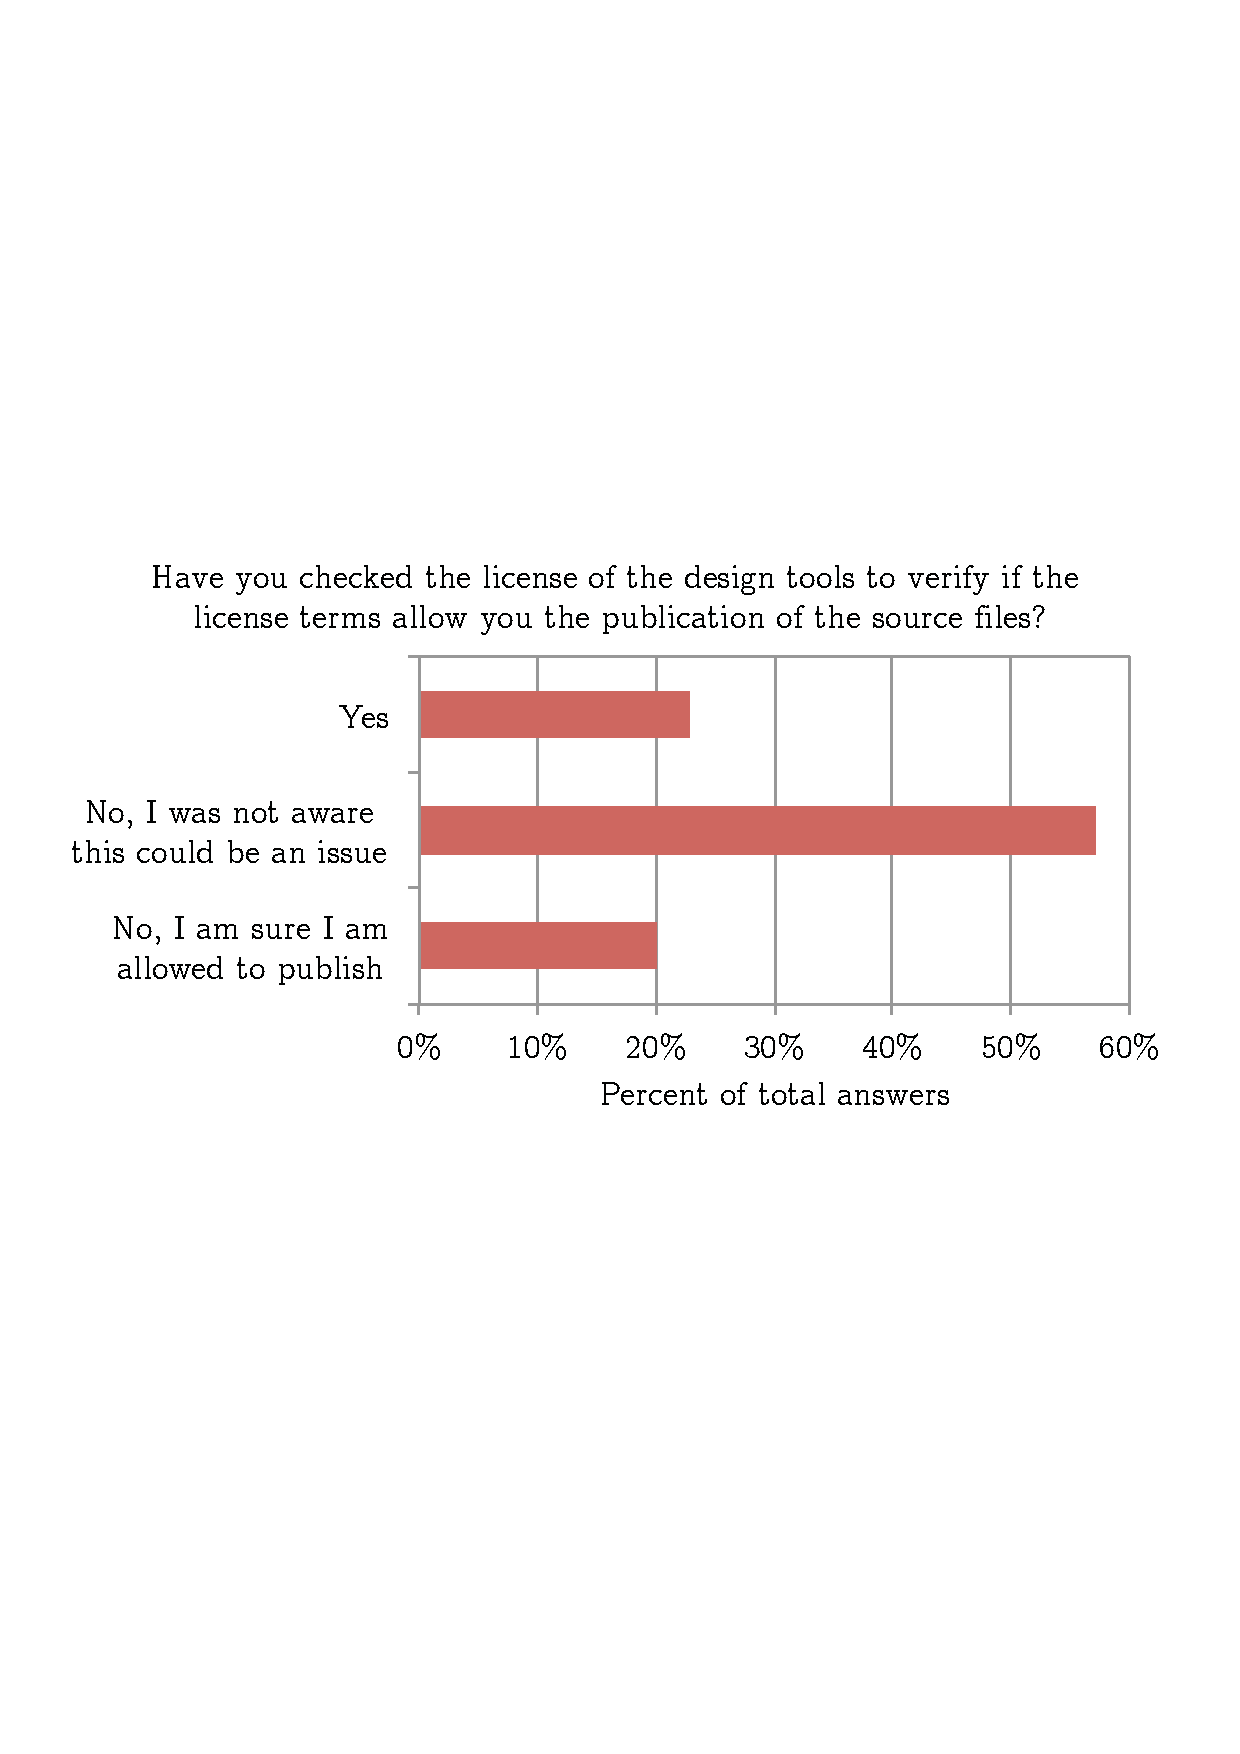
\includegraphics[width=\columnwidth]{figures/checklicense}
\caption{Awareness about CAD tool licenses limitations by people participating to the survey.}
\label{fig:aware}
\end{figure}

To clarify this issue we contacted twelve of the major editors of mechanical CAD and PCB routing software.
We asked them if their educational license allows the publication of the source files, and we specified that the published files could have been downloaded by a company to produce the system for commercial purposes.
Figure~\ref{fig:editors} summarizes the result of this survey.
Only three of the twelve editors have education licenses allowing this type of publication. 
Two others explicitly mentioned the possibility to ask for permission before publication.
A large mechanical CAD editor was puzzled by our questions and after realizing the impact of the license, introduced a special condition allowing publication of files in clearly labeled open source hardware projects.
In previous situations of open source publication, the same editor asked the universities to purchase commercial licenses to permit publication.
This can multiply by a factor of some hundreds the price of the CAD license.
This blocking factor for open hardware also applies to the publication of scientific results, as promoted by many governments in the last decade and generally called ``open science''.
The change of policy in CAD files publication that we obtained is a sign of the very positive trend set by open hardware and by open science in general.

\begin{figure}
\centering
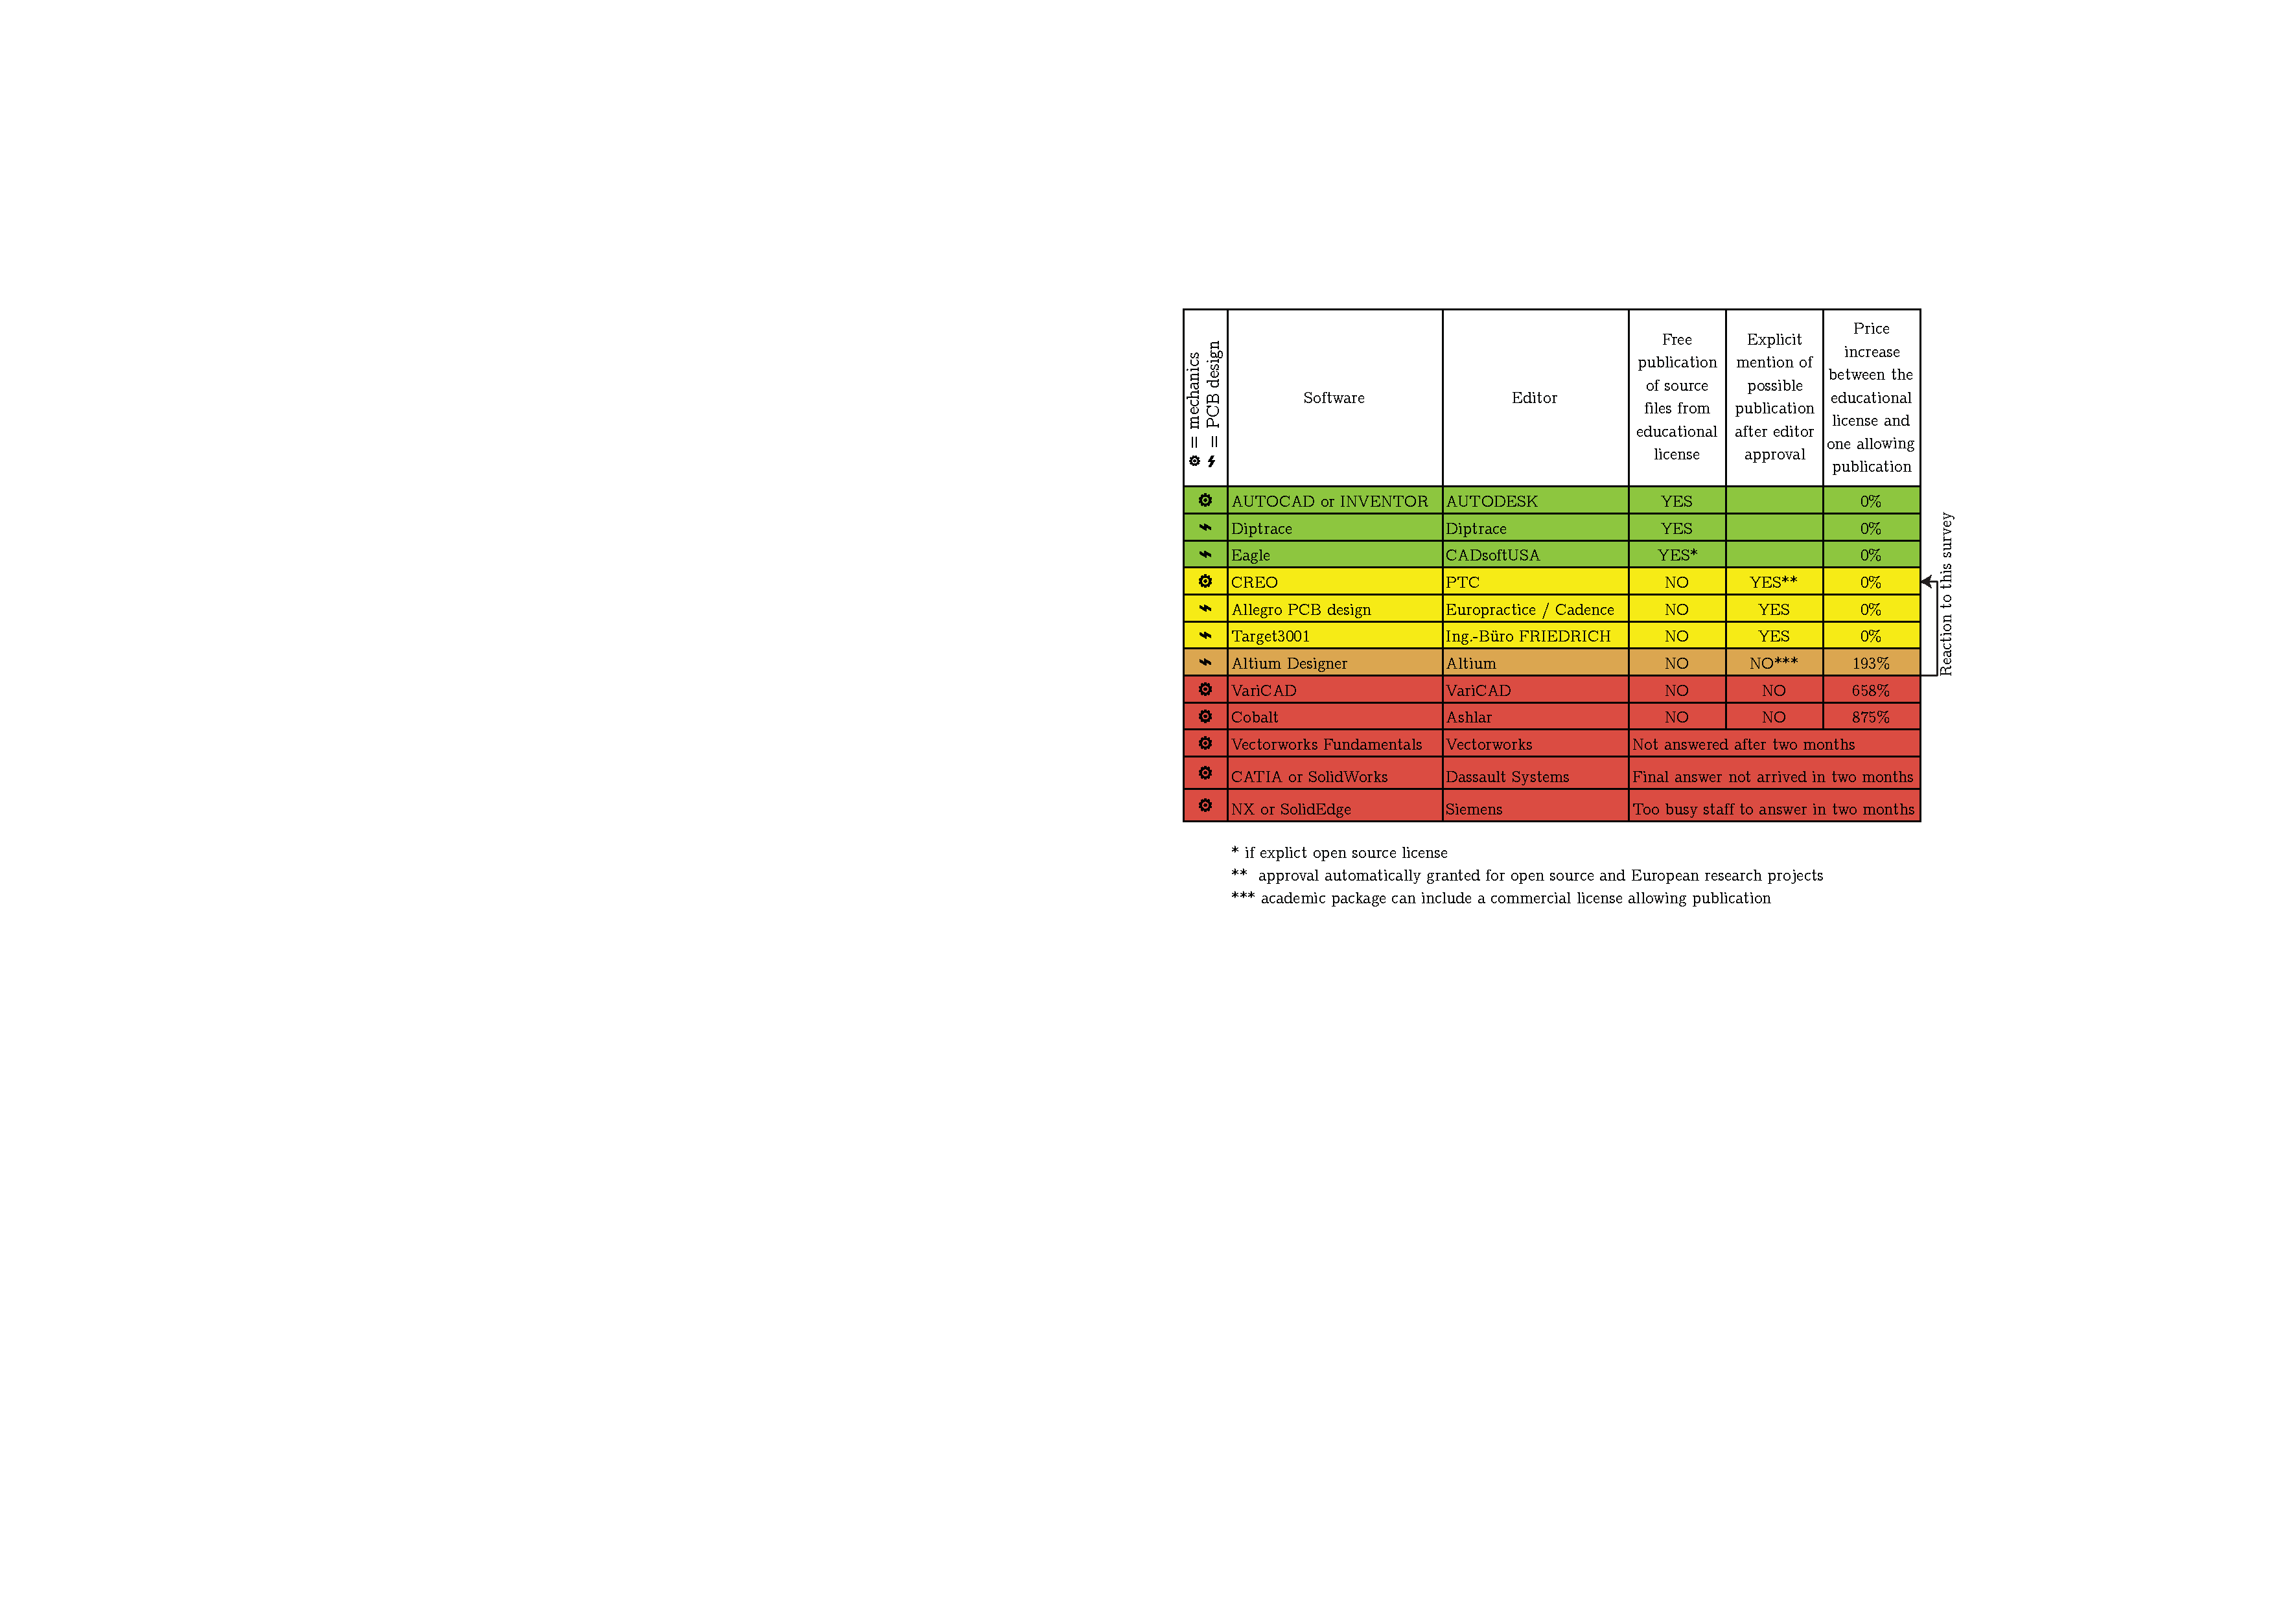
\includegraphics[width=\columnwidth]{figures/table}
\caption{Publication possibilities as function of the CAD editors, situation end of March 2016.}
\label{fig:editors}
\end{figure}

As a conclusion, this legal issue is totally underestimated by both people participating to the projects and by the CAD editors. 
In a period where editors are looking for additional revenues and are attacking universities for misuse of licenses\footnote{We are aware, just in Switzerland, of two situations where large amounts of money are asked to universities for non-respect of software licenses.}, this can be a very dangerous situation.

\subsection{Who designs and produces the hardware}

Among the fundamental choices when starting an open source hardware project, there is the choice of the type of production. 
In the definition of open hardware we gave, it is stated that one should offer an ``hardware whose design is made publicly available so that anyone can ... make... the ... hardware ''.
Behind the ``anyone'' should we consider every single person or only companies able to produce the product?
This choice has implications on who designs the system and how.
In our project we have two different types of hardware: the robot itself and the accessories used in specific activities.
The robot is the expensive part and has a very neutral design, allowing adaptation to specific situations.
This adaptation is achieved by custom accessories that increase the attraction of the robot in its specific role, enabling activity for different ages and genders.

For the robot itself we opted for the second interpretation of the definition, considering under ``anyone'' only the professional structures able to mass-produce hardware, for a reason of price and complexity of the product. 
When looking for the best performance per price ratio, we decided to use techniques that require heavy equipment.
For instance we decided to produce all mechanical parts by injection molds. 
This ensures a price per part of some cents, which cannot be achieved by others techniques.
Letting end-user produce their own parts would results in higher prices for less performances. 
This choice has another implication: only a core team of highly skilled engineers can contribute to the project. 
It is not trivial to design a mechanical part that can be molded in the simplest possible way.

For the accessories, less technically challenging and stronger linked with creativity and educational value, we promoted techniques that are accessible to ``anyone'' in the broader sense: paper, cardboard, LEGO\textsuperscript{\textregistered} constructions and 3D printing, as explained in section~\ref{sec:crea} and illustrated in Figure~\ref{fig:example-construction}.
This allows a much broader spectrum of contributor, especially among the teachers.


\begin{figure}
\centering
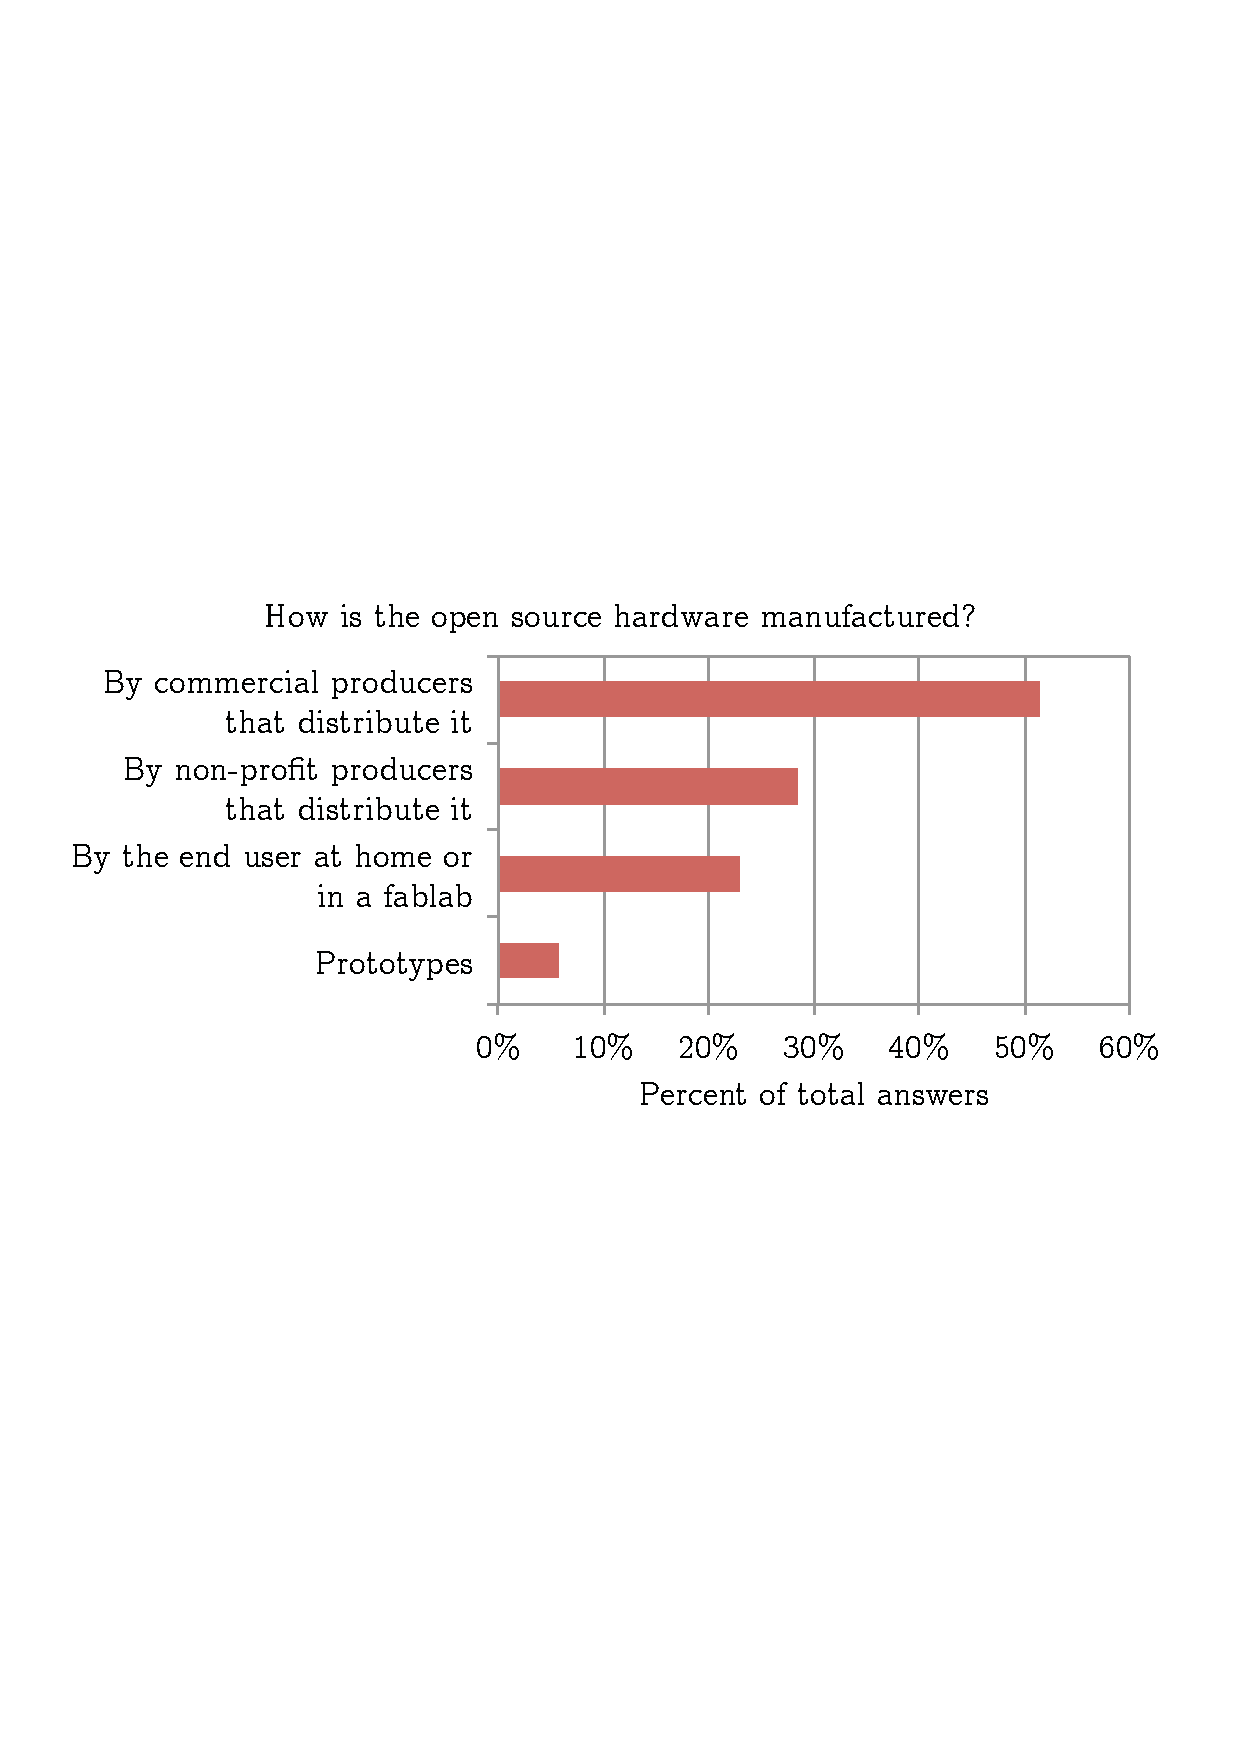
\includegraphics[width=\columnwidth]{figures/manufacturing}
\caption{Production methods in the projects mentioned by the people participating to the survey.}
\label{fig:production}
\end{figure}

When looking at the results of the survey (see Figure~\ref{fig:production}), we can observe that the most common production method is a centralized one by commercial companies.
Indeed, large open source hardware projects like Arduino are based on this model.
One could advocate that this choice of central production and sale of hardware can bring these robotic projects closer to standard commercial models, ending in users not involved in the project and not feeling close to the developers.
In our case we decided to counterbalance this apparently business oriented model by creating a non-profit association, called Mobsya, in charge of producing and selling the robots. 
This is also a very well represented production method in our survey.
Of course anybody else could produce the Thymio based on more buiness-oriented models, but at least the initial production has been done respecting a coherent and global non-profit strategy, in line with educational values of the community of users.
Moreover the user are better integrated is the second layer of open source hardware consisting in accessories, where anybody can contribute with own designs.

Another strong difference between a standard consumer product and our vision of open hardware, is that Thymio should be durable.
Schools do not have large budget for technological tools and make strong investment in training of their teachers when adopting a new tool.
Therefore the lifetime of the products should be as long as possible. 
The open hardware approach gives to the user, or to a generic technician, better conditions to repair the system.
Supporting this type of operation has an impact on the robot design; for instance Thymio can be easily opened with four standard screws, and we introduced connectors between key elements such as motors, speaker, or the battery and the main printed circuit. 

Another key element in supporting repair by the users are the calibration methods. 
When choosing very low cost components, one gets into large dispersion of the characteristics. 
In our case, for instance, the right and left wheel motors can have very different electrical characteristics, resulting in different speed evaluations and therefore in the robot not going straight when the two motors regulators have the same set speed.
To correct this problem, one interesting solution is to introduce factory calibration, storing correction factors that are specific for each robot, in the microcontroller memory. 
To allow the user to replace a broken motor, it is essential to give him also the possibility to re-calibrate the robot and adjust the parameters of the new motors.
In Thymio, this results in the design and the documentation of calibration processes that can be performed by anyone, getting close to the original definition of open source hardware.

\subsection{Added value of open source hardware in distribution}

Beside the sale of more than 10'000 robots by a non-profit organization producing it, there are several elements that show a specific advantage of having chosen an open source hardware model.

The first element is linked to the financial support of the project.
Although the non-profit nature of the project blocked the possibility to have shareholders injecting capital, this same nature enabled a lot of institutional donations linked with the societal goal of the project.
The financial support through donations instead of acquisition of shares, allows keeping a total decisional freedom and void debts at the same time.
The main disadvantage of this approach is the amount of financial support, limited in our case of several hundreds of thousands of dollars. 

The second interesting element of the open source hardware appraoch is the very high acceptance of the resulting robot by universities and their offices in charge of promotion of science.
Although these are not the primary user targeted by the robot, these are institutions with high visibility and influence on school programs. 
In particular INRIA in France and the University of Cambridge in he United Kingdoms decided to use Thymio as tool for promotion of their activities and introduced it into schools.
In France, INRIA developed several teaching modules and supported the training of more than 1000 teachers to the use of this particular robot. 
This finally resulted in having the Thymio robot included as one of the tools chosen for the education of digital science in the reference books of the French Academy of Science and its foundation for promotion of science in education, called ``La main \`a la p\^ate.''
The fact that Thymio is open source allows these institution to have a better control on the tool they use, as they can ensure maintenance and even further development of it. 
The impulsion given by the academic institutions has been followed by many teachers who contributed with own teaching material. 
Up to date one can find more than 50 teaching modules, one large tutorial, and many reports on school activities using Thymio. 

In some cases, the open source nature of this project was a crucial political argument for the choice of this platform.
In the state of Geneva, for instance, the government decided to move toward open source non-proprietary tools in education.
All primary school- and most secondary school computers have been installed with the Ubuntu distribution of Linux. 
On this operating system the LEGO\textsuperscript{\textregistered} Mindstorms\textsuperscript{\textregistered} software tools are not available, and their proprietary nature is not compatible with the philosophy dictated by the government. 
Thymio was therefore extremely welcome, and the state of Geneva organized own training courses for teachers, ported several educational materials into their curriculum and organized a lending system for all schools that cannot afford to buy the robots.
Others states are starting following this model.

Finally the non-profit nature of the project, including the production infrastructure, has contributed to reduce the obstacle toward the acquisition of this platform for many schools, where teachers have a strong societal motivation and are reluctant to use tax-payers money to pay the divident of some shareholders.

\subsection{Problems of open-source projects}

\begin{figure}
\centering
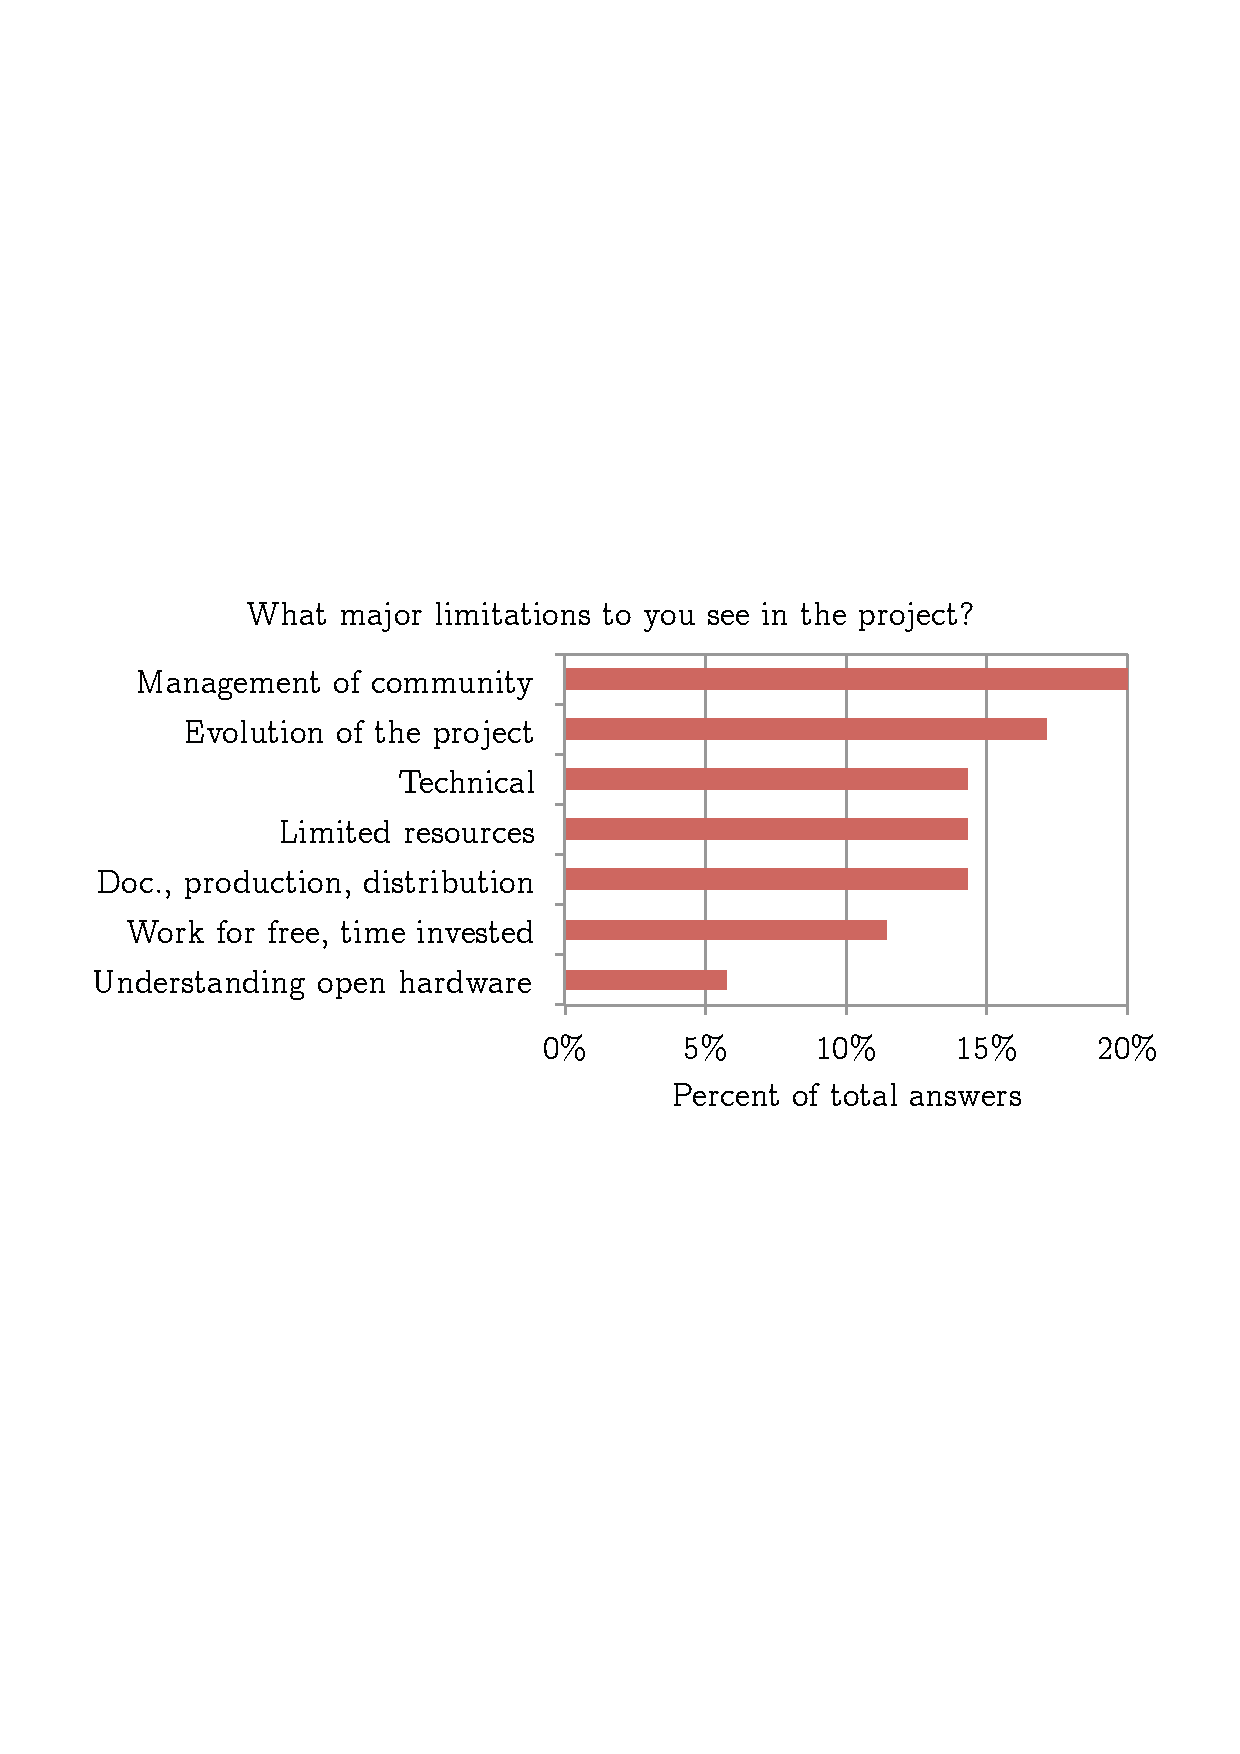
\includegraphics[width=\columnwidth]{figures/limitations}
\caption{Limitations of open source hardware projects observed by participants to open source hardware projects.}
\label{fig:problems}
\end{figure}

The very specific structure of an open project has also drawbacks. 
Asked about problems met in their project (see Figure~\ref{fig:problems}), the participants to our survey mention the management of the community, the evolution of the project, the efforts in documentation, production and distribution and the limited resources.
There are here two kind of problems: one of management of people, the other in the development of the project after the first design.
The management of the project seems a recurrent problem and is related to the nature of this type of structure, mainly very flat and built on academic people with engineering background. 
More than 62\% of the answers to our survey report about projects that are managed by the founder of the initiative and not by the most expert in the field or by a manager, which is perhaps not the best objective choice.
It is indeed very difficult to evolve from a phase where the engineering is the core of the project, to a new phase where communication and management play an increasing role.
The same holds for several other factors, like the efforts in documentation, production and distribution of the product. 
Also here there is a change of activity from the very creative and appealing design phase, to a phase of documentation and, in some cases, production and distribution which is not at all the same type of activity and requires different skills.
This shift requires extra efforts and motivation, which are often missing, especially for activities like documentation that are not appreciated by engineers.
In general many respondents to our survey identified the evolution of the project as a general problematic issue, which summarizes the several aspects mentioned above.

In the Thymio project we had very similar issues and tried to address them by having several partners, each of them specialized in one aspect: design, production and sale, creation of educational material, etc.
Despite this approach, we had also problems of management of the community, and issues in finding the right long term vision, especially having so many partners. 
The long term vision of a sales person is not the same of an engineer, and those confrontation result in conflicts in a community with a very flat hierarchy. 
A key element that allowed to keep cohesion in our community was to share, among all partners, strong basic values about improvement of society through education.


\section{Conclusion}

The introduction of robots in formal education is a very challenging task, not only because of technical requirements such as low cost, performances and interactivity, but also because of factors depending on the school environment, such as the diversity of the educational programs, the dependence on local structures and languages, or the required training of teachers.
Most of the current robotic tools for education capitalize upon existing hardware platforms, programming environments, or robot architectures.
Because they do not consider all elements at stake, these tools fail to meet some challenges of the field.
On the contrary, in this paper we presented a global approach that tackles these questions in a holistic way, based on open source and non-profit principles.
The result is the Thymio robot and its surrounding open source community including engineers, art designers, production and sales people, and teachers.
The open source hardware and the related contributions are split in two categories: the robot itself, produced by a non-profit organization and requiring very advanced skills in both design and production, and the accessories for activities, based on techniques broadly accessible and with a larger panel of contributors.

The open source hardware development and dissemination of Thymio addresses several of the issues found in educational robotics.
It allowed to broadly distribute the robot with minimal changes dues to management of intellectual properties, royalties, financial support and so on.
This was achieved with an excellent match between the philosophy of the project and the one of the community of users in education.
In particular, the open source approach allows to provide a durable robot, easy to maintain and repair, with at the same time a community of users providing educational material and mutual support.

By making a survey among a panel of people contributing to open source hardware projects, we could observe that our project shares some characteristics with the majority of the projects represented in the survey. 
We also had problems of management of the community, we chose production and distributions methods that are broadly applied, and we share most of the motivation elements that are behind other projects.
We identified an underestimated legal issue for open source hardware projects in the licensing term of CAD software.
Indeed only very few editors have licenses allowing the publication of source files created with educational license.
Two surveys among the users and the CAD editors shows that both people contributing or leading open source hardware projects and the editors themselves are now aware of this issue.
Finally we could show some elements that differentiate our project from other open source hardware ones, being specific to educational robotics.
In particular our project takes advantage from an alignment between the principles underlying open source project and the nature of education institutions. 
This fits with a political trend toward open source in education and in science in general.
We also found a solution to the struggling question of production methods by splitting our hardware in two categories, enabling both very advanced hardware and inclusion of a broad community of end users.
This addresses durability of equipment and gender issues that are critical in education.

\bibliography{ThymioEdu}
\bibliographystyle{ieeetr}

%-\addtolength{\textheight}{-12cm}   % This command serves to balance the column lengths
                                  % on the last page of the document manually. It shortens
                                  % the textheight of the last page by a suitable amount.
                                  % This command does not take effect until the next page
                                  % so it should come on the page before the last. Make
                                  % sure that you do not shorten the textheight too much.

%%%%%%%%%%%%%%%%%%%%%%%%%%%%%%%%%%%%%%%%%%%%%%%%%%%%%%%%%%%%%%%%%%%%%%%%%%%%%%%%



%%%%%%%%%%%%%%%%%%%%%%%%%%%%%%%%%%%%%%%%%%%%%%%%%%%%%%%%%%%%%%%%%%%%%%%%%%%%%%%%



%%%%%%%%%%%%%%%%%%%%%%%%%%%%%%%%%%%%%%%%%%%%%%%%%%%%%%%%%%%%%%%%%%%%%%%%%%%%%%%%
%\section*{APPENDIX}
%
%questionnaire?
%
%\section*{ACKNOWLEDGMENT}
%
%??



%%%%%%%%%%%%%%%%%%%%%%%%%%%%%%%%%%%%%%%%%%%%%%%%%%%%%%%%%%%%%%%%%%%%%%%%%%%%%%%%


\end{document}
